% Options for packages loaded elsewhere
\PassOptionsToPackage{unicode}{hyperref}
\PassOptionsToPackage{hyphens}{url}
\PassOptionsToPackage{dvipsnames,svgnames,x11names}{xcolor}
%
\documentclass[
  12pt,
]{book}
\usepackage{amsmath,amssymb}
\usepackage{iftex}
\ifPDFTeX
  \usepackage[T1]{fontenc}
  \usepackage[utf8]{inputenc}
  \usepackage{textcomp} % provide euro and other symbols
\else % if luatex or xetex
  \usepackage{unicode-math} % this also loads fontspec
  \defaultfontfeatures{Scale=MatchLowercase}
  \defaultfontfeatures[\rmfamily]{Ligatures=TeX,Scale=1}
\fi
\usepackage{lmodern}
\ifPDFTeX\else
  % xetex/luatex font selection
\fi
% Use upquote if available, for straight quotes in verbatim environments
\IfFileExists{upquote.sty}{\usepackage{upquote}}{}
\IfFileExists{microtype.sty}{% use microtype if available
  \usepackage[]{microtype}
  \UseMicrotypeSet[protrusion]{basicmath} % disable protrusion for tt fonts
}{}
\makeatletter
\@ifundefined{KOMAClassName}{% if non-KOMA class
  \IfFileExists{parskip.sty}{%
    \usepackage{parskip}
  }{% else
    \setlength{\parindent}{0pt}
    \setlength{\parskip}{6pt plus 2pt minus 1pt}}
}{% if KOMA class
  \KOMAoptions{parskip=half}}
\makeatother
\usepackage{xcolor}
\usepackage[margin = 3cm]{geometry}
\usepackage{color}
\usepackage{fancyvrb}
\newcommand{\VerbBar}{|}
\newcommand{\VERB}{\Verb[commandchars=\\\{\}]}
\DefineVerbatimEnvironment{Highlighting}{Verbatim}{commandchars=\\\{\}}
% Add ',fontsize=\small' for more characters per line
\usepackage{framed}
\definecolor{shadecolor}{RGB}{248,248,248}
\newenvironment{Shaded}{\begin{snugshade}}{\end{snugshade}}
\newcommand{\AlertTok}[1]{\textcolor[rgb]{0.94,0.16,0.16}{#1}}
\newcommand{\AnnotationTok}[1]{\textcolor[rgb]{0.56,0.35,0.01}{\textbf{\textit{#1}}}}
\newcommand{\AttributeTok}[1]{\textcolor[rgb]{0.13,0.29,0.53}{#1}}
\newcommand{\BaseNTok}[1]{\textcolor[rgb]{0.00,0.00,0.81}{#1}}
\newcommand{\BuiltInTok}[1]{#1}
\newcommand{\CharTok}[1]{\textcolor[rgb]{0.31,0.60,0.02}{#1}}
\newcommand{\CommentTok}[1]{\textcolor[rgb]{0.56,0.35,0.01}{\textit{#1}}}
\newcommand{\CommentVarTok}[1]{\textcolor[rgb]{0.56,0.35,0.01}{\textbf{\textit{#1}}}}
\newcommand{\ConstantTok}[1]{\textcolor[rgb]{0.56,0.35,0.01}{#1}}
\newcommand{\ControlFlowTok}[1]{\textcolor[rgb]{0.13,0.29,0.53}{\textbf{#1}}}
\newcommand{\DataTypeTok}[1]{\textcolor[rgb]{0.13,0.29,0.53}{#1}}
\newcommand{\DecValTok}[1]{\textcolor[rgb]{0.00,0.00,0.81}{#1}}
\newcommand{\DocumentationTok}[1]{\textcolor[rgb]{0.56,0.35,0.01}{\textbf{\textit{#1}}}}
\newcommand{\ErrorTok}[1]{\textcolor[rgb]{0.64,0.00,0.00}{\textbf{#1}}}
\newcommand{\ExtensionTok}[1]{#1}
\newcommand{\FloatTok}[1]{\textcolor[rgb]{0.00,0.00,0.81}{#1}}
\newcommand{\FunctionTok}[1]{\textcolor[rgb]{0.13,0.29,0.53}{\textbf{#1}}}
\newcommand{\ImportTok}[1]{#1}
\newcommand{\InformationTok}[1]{\textcolor[rgb]{0.56,0.35,0.01}{\textbf{\textit{#1}}}}
\newcommand{\KeywordTok}[1]{\textcolor[rgb]{0.13,0.29,0.53}{\textbf{#1}}}
\newcommand{\NormalTok}[1]{#1}
\newcommand{\OperatorTok}[1]{\textcolor[rgb]{0.81,0.36,0.00}{\textbf{#1}}}
\newcommand{\OtherTok}[1]{\textcolor[rgb]{0.56,0.35,0.01}{#1}}
\newcommand{\PreprocessorTok}[1]{\textcolor[rgb]{0.56,0.35,0.01}{\textit{#1}}}
\newcommand{\RegionMarkerTok}[1]{#1}
\newcommand{\SpecialCharTok}[1]{\textcolor[rgb]{0.81,0.36,0.00}{\textbf{#1}}}
\newcommand{\SpecialStringTok}[1]{\textcolor[rgb]{0.31,0.60,0.02}{#1}}
\newcommand{\StringTok}[1]{\textcolor[rgb]{0.31,0.60,0.02}{#1}}
\newcommand{\VariableTok}[1]{\textcolor[rgb]{0.00,0.00,0.00}{#1}}
\newcommand{\VerbatimStringTok}[1]{\textcolor[rgb]{0.31,0.60,0.02}{#1}}
\newcommand{\WarningTok}[1]{\textcolor[rgb]{0.56,0.35,0.01}{\textbf{\textit{#1}}}}
\usepackage{longtable,booktabs,array}
\usepackage{calc} % for calculating minipage widths
% Correct order of tables after \paragraph or \subparagraph
\usepackage{etoolbox}
\makeatletter
\patchcmd\longtable{\par}{\if@noskipsec\mbox{}\fi\par}{}{}
\makeatother
% Allow footnotes in longtable head/foot
\IfFileExists{footnotehyper.sty}{\usepackage{footnotehyper}}{\usepackage{footnote}}
\makesavenoteenv{longtable}
\usepackage{graphicx}
\makeatletter
\newsavebox\pandoc@box
\newcommand*\pandocbounded[1]{% scales image to fit in text height/width
  \sbox\pandoc@box{#1}%
  \Gscale@div\@tempa{\textheight}{\dimexpr\ht\pandoc@box+\dp\pandoc@box\relax}%
  \Gscale@div\@tempb{\linewidth}{\wd\pandoc@box}%
  \ifdim\@tempb\p@<\@tempa\p@\let\@tempa\@tempb\fi% select the smaller of both
  \ifdim\@tempa\p@<\p@\scalebox{\@tempa}{\usebox\pandoc@box}%
  \else\usebox{\pandoc@box}%
  \fi%
}
% Set default figure placement to htbp
\def\fps@figure{htbp}
\makeatother
\setlength{\emergencystretch}{3em} % prevent overfull lines
\providecommand{\tightlist}{%
  \setlength{\itemsep}{0pt}\setlength{\parskip}{0pt}}
\setcounter{secnumdepth}{5}
\ifLuaTeX
\usepackage[bidi=basic]{babel}
\else
\usepackage[bidi=default]{babel}
\fi
\babelprovide[main,import]{spanish}
% get rid of language-specific shorthands (see #6817):
\let\LanguageShortHands\languageshorthands
\def\languageshorthands#1{}
\usepackage{setspace}
%\linespread{1.5}
%\usepackage{tikz}
%\usetikzlibrary{shapes,arrows}
\usepackage{pdflscape}
\newcommand{\blandscape}{\begin{landscape}}
\newcommand{\elandscape}{\end{landscape}}
\renewcommand{\thesection}{\Roman{section}}
\renewcommand{\thesubsection}{\Alph{subsection}}
\usepackage{booktabs}
\usepackage{amsthm}
\makeatletter
\def\thm@space@setup{%
  \thm@preskip=8pt plus 2pt minus 4pt
  \thm@postskip=\thm@preskip
}
\makeatother
\usepackage{amsmath}
\usepackage[ruled,vlined,linesnumbered]{algorithm2e}
\usepackage{tabularray}
\usepackage[]{natbib}
\bibliographystyle{apalike}
\usepackage{bookmark}
\IfFileExists{xurl.sty}{\usepackage{xurl}}{} % add URL line breaks if available
\urlstyle{same}
\hypersetup{
  pdftitle={Análisis de encuestas con R},
  pdfauthor={Andrés Gutiérrez,Stalyn Guerrero, Cristian Téllez, Giovany Babativa},
  pdflang={es},
  colorlinks=true,
  linkcolor={blue},
  filecolor={Maroon},
  citecolor={Blue},
  urlcolor={Blue},
  pdfcreator={LaTeX via pandoc}}

\title{Análisis de encuestas con R}
\author{Andrés Gutiérrez\footnote{Experto Regional en Estadísticas Sociales - Comisión Económica para América Latina y el Caribe (CEPAL) - \href{mailto:andres.gutierrez@cepal.org}{\nolinkurl{andres.gutierrez@cepal.org}}},Stalyn Guerrero\footnote{Consultor - Comisión Económica para América Latina y el Caribe (CEPAL), \href{mailto:guerrerostalyn@gmail.com}{\nolinkurl{guerrerostalyn@gmail.com}}}, Cristian Téllez\footnote{Consultor - Comisión Económica para América Latina y el Caribe (CEPAL), \href{mailto:cftellezp@unal.edu.co}{\nolinkurl{cftellezp@unal.edu.co}}}, Giovany Babativa\footnote{Consultor - Comisión Económica para América Latina y el Caribe (CEPAL), \href{mailto:gbabativam@gmail.com}{\nolinkurl{gbabativam@gmail.com}}}}
\date{2025-09-25}

\begin{document}
\maketitle

{
\hypersetup{linkcolor=}
\setcounter{tocdepth}{1}
\tableofcontents
}
\listoffigures
\listoftables
\chapter*{Prefacio}\label{prefacio}
\addcontentsline{toc}{chapter}{Prefacio}

La versión online de este libro está licenciada bajo una \href{http://creativecommons.org/licenses/by-nc-sa/4.0/}{Licencia Internacional de Creative Commons para compartir con atribución no comercial 4.0}.

Este libro es el resultado de un compendio de las experiencias internacionales prácticas adquiridas por el autor como Experto Regional en Estadísticas Sociales de la CEPAL.

\chapter{Análisis de las variables continuas en encuestas de hogares}\label{anuxe1lisis-de-las-variables-continuas-en-encuestas-de-hogares}

Los desarrollos estadísticos están en permanente evolución, surgiendo nuevas metodologías y desarrollando nuevos enfoques en el análisis de encuestas. Estos desarrollos parten de la academia, luego son adoptados por las empresas (privadas o estatales) y entidades estatales, las cuales crean la necesidad que estos desarrollos sean incluidos en software estadísticos licenciados, proceso que puede llevar mucho tiempo.

Algunos investigadores para acortar los tiempos y poner al servicio de la comunidad sus descubrimientos y desarrollos, hacen la implementación de sus metodologías en paquetes estadísticos de código abierto como \textbf{R} o \textbf{Python}. Teniendo \textbf{R} un mayor número de desarrollos en el procesamiento de las encuestas.

Como se ha venido mencionando anteriormente, dentro del software \emph{R} se disponen de múltiples librerías para el procesamiento de encuestas, estas varían dependiendo del enfoque de programación desarrollado por el autor o la necesidad que se busque suplir. Como es el objetivo de este libro y como se ha venido trabajando en los capítulos anteriores nos centraremos en las libreria \texttt{survey} y \texttt{srvyr}. Se incluiran más librerías de acuerdo a las necesidades que se presenten.

\section{Lectura de bases de datos y definición del diseño muestral}\label{lectura-de-bases-de-datos-y-definiciuxf3n-del-diseuxf1o-muestral}

Las bases de datos (tablas de datos) pueden estar disponibles en una variedad de formatos (.xlsx, .dat, .csv, .sav, .txt, etc.). Sin embargo, por experiencia es recomendable leer cualquiera de estos formatos y proceder inmediatamente a guardarlos en un archivo de extensión \texttt{.rds}, que es nativa de R. Los archivos \texttt{.rds} permiten almacenar cualquier objeto o información en R, como marcos de datos, vectores, matrices, listas, entre otros. Se caracterizan por su flexibilidad y compatibilidad completa con R, lo que facilita su reutilización en análisis posteriores.

Por otro lado, existen otros tipos de archivos propios de R, como \texttt{.Rdata}. La diferencia principal es que los archivos \texttt{.rds} contienen un solo objeto, mientras que \texttt{.Rdata} puede almacenar múltiples objetos. Por ello, se recomienda trabajar preferentemente con archivos \texttt{.rds}.

Para ejemplificar la sintaxis que se utilizará en R, se tomará la misma base del capítulo anterior, que contiene una muestra de 2,427 registros y proviene de un muestreo complejo. A continuación, se muestra cómo cargar un archivo con extensión \texttt{.rds}:

\begin{Shaded}
\begin{Highlighting}[]
\FunctionTok{library}\NormalTok{(tidyverse)}

\NormalTok{encuesta }\OtherTok{\textless{}{-}} \FunctionTok{readRDS}\NormalTok{(}\StringTok{"Data/encuesta.rds"}\NormalTok{)}
\FunctionTok{head}\NormalTok{(encuesta)}
\end{Highlighting}
\end{Shaded}

\begin{verbatim}
##        HHID   Stratum NIh nIh  dI PersonID     PSU  Zone    Sex Age MaritalST
## 1 idHH00031 idStrt001   9   2 4.5  idPer01 PSU0003 Rural   Male  68   Married
## 2 idHH00031 idStrt001   9   2 4.5  idPer02 PSU0003 Rural Female  56   Married
## 3 idHH00031 idStrt001   9   2 4.5  idPer03 PSU0003 Rural Female  24   Married
## 4 idHH00031 idStrt001   9   2 4.5  idPer04 PSU0003 Rural   Male  26   Married
## 5 idHH00031 idStrt001   9   2 4.5  idPer05 PSU0003 Rural Female   3      <NA>
## 6 idHH00041 idStrt001   9   2 4.5  idPer01 PSU0003 Rural Female  61   Widowed
##   Income Expenditure Employment Poverty dki dk       wk Region    CatAge
## 1 409.87      346.34   Employed NotPoor   8 36 34.50371  Norte Más de 60
## 2 409.87      346.34   Employed NotPoor   8 36 33.63761  Norte     46-60
## 3 409.87      346.34   Employed NotPoor   8 36 33.63761  Norte     16-30
## 4 409.87      346.34   Employed NotPoor   8 36 34.50371  Norte     16-30
## 5 409.87      346.34       <NA> NotPoor   8 36 33.63761  Norte       0-5
## 6 823.75      392.24   Employed NotPoor   8 36 33.63761  Norte Más de 60
\end{verbatim}

Según Naciones Unidas (2005, sec.~7.8), es fundamental que la estructura de los diseños de muestreo complejos se tenga en cuenta en el proceso de inferencia al estimar estadísticas oficiales basadas en encuestas de hogares. Ignorar este aspecto puede generar estimaciones sesgadas y errores de muestreo subestimados. En este contexto, los programas estadísticos ofrecen funcionalidades clave para el manejo de datos provenientes de este tipo de diseños (Heeringa, West y Berglund, 2017, Apéndice A).

De manera general, herramientas estadísticas como \textbf{R, Stata, SAS y SPSS} cuentan con módulos y bibliotecas que optimizan la estimación de varianzas en muestras complejas, incorporando métodos de replicación para varianzas basadas en el diseño. Mientras que R es de acceso libre, los otros programas requieren licencias de pago. Estas plataformas permiten calcular estadísticas descriptivas (medias, totales, proporciones, percentiles, razones) y ajustar modelos de regresión considerando la estructura del diseño de la encuesta. Los programas especializados generan automáticamente el efecto del diseño, facilitando la interpretación de la variabilidad de las estimaciones.

El uso de estos paquetes implica que el usuario suministre información clave del diseño muestral, como factores de expansión, estratificación e identificadores de conglomerados. A continuación, se ofrece un resumen general, aunque no exhaustivo, de las funciones y posibilidades que brindan los principales programas estadísticos para el análisis de encuestas complejas.

Una vez cargada la muestra de hogares en \texttt{R}, el siguiente paso es definir el diseño muestral del cual proviene dicha muestra. Para ello se utilizará el paquete \texttt{srvyr}, que como se mencionó anteriormente, surge como un complemento de \texttt{survey}. Estas librerías permiten definir objetos tipo \textbf{survey.design}, a los que se aplican las funciones de estimación y análisis de encuestas, y que pueden ser combinadas con la programación de tubería (\texttt{\%\textgreater{}\%}) del paquete \texttt{tidyverse}.

A manera de ejemplificar los conceptos mencionados, a continuación se define en \texttt{R} el diseño de muestreo del cual proviene la muestra contenida en el objeto \textbf{encuesta}:

\begin{Shaded}
\begin{Highlighting}[]
\FunctionTok{options}\NormalTok{(}\AttributeTok{survey.lonely.psu =} \StringTok{"adjust"}\NormalTok{) }

\FunctionTok{library}\NormalTok{(srvyr)}

\NormalTok{diseno }\OtherTok{\textless{}{-}}\NormalTok{ encuesta }\SpecialCharTok{\%\textgreater{}\%} 
  \FunctionTok{as\_survey\_design}\NormalTok{(}
    \AttributeTok{strata =}\NormalTok{ Stratum,  }
    \AttributeTok{ids =}\NormalTok{ PSU,        }
    \AttributeTok{weights =}\NormalTok{ wk,      }
    \AttributeTok{nest =}\NormalTok{ T)}
\end{Highlighting}
\end{Shaded}

En el código anterior se puede observar que, en primera instancia se debe definir la base de datos en la cual se encuentra la muestra seleccionada. Seguido de eso, se debe definir el tipo de objeto en \texttt{R} con el cual se trabajará, para nuestro caso, será un objeto \emph{survey\_design} el cual se define usando la función \emph{as\_survey\_design}. ahora bien, una vez definido el tipo de objeto se procede a definir los parámetros del diseño definido. Para este caso fue un diseño de muestreo estratificado y en varias etapas. Estos argumentos se definen dentro de la función \emph{as\_survey\_design} como sigue. Para definir los estratos de utiliza el argumento \emph{strata} y se define en qué columna están los estratos en mi base de datos. Ahora bien, para definir las UPM´s, en el argumento \emph{ids} se definen la columna donde se encuntran los conglomerados seleccionados en la primera etapa. También, se definen los pesos de muestreo en el argumento \emph{weights} y, por último, con el argumento \emph{nest=T} se define que las UPM´s están dentro de los estratos.

\section{Análisis gráfico: Histogramas y Boxplot}\label{anuxe1lisis-gruxe1fico-histogramas-y-boxplot}

Una vez cargada la muestra a \texttt{R} y definido el diseño muestral del cual proviene se pueden hacer los primeros análisis. Como es natural, se inician con análisis gráficos. A continuación, se muestran los códigos computacionales con los cuales se hacen histogramas en \texttt{R} para la variable ingresos teniendo en cuenta el diseño muestral y los factores de expansión haciendo uso la función \texttt{svyhist} de la librería \texttt{survey}.

\begin{Shaded}
\begin{Highlighting}[]
\FunctionTok{library}\NormalTok{(survey)}
\FunctionTok{library}\NormalTok{(srvyr)}
\FunctionTok{svyhist}\NormalTok{(}
  \SpecialCharTok{\textasciitilde{}}\NormalTok{ Income ,}
\NormalTok{  diseno,}
  \AttributeTok{main =} \StringTok{"Ingresos por hogar"}\NormalTok{,}
  \AttributeTok{col =} \StringTok{"grey80"}\NormalTok{,}
  \AttributeTok{xlab =} \StringTok{"Ingreso"}\NormalTok{,}
  \AttributeTok{probability =} \ConstantTok{FALSE}
\NormalTok{)}
\end{Highlighting}
\end{Shaded}

\pandocbounded{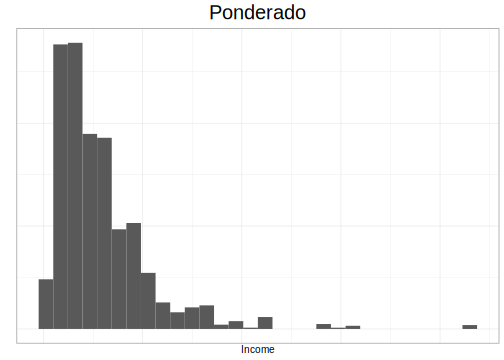
\includegraphics[keepaspectratio]{04-Continuas_files/figure-latex/hist1-1.pdf}}

Como se pudo observar en el código anterior, para generar un histograma teniendo en cuenta el diseño muestral se usó la función \texttt{svyhist}. En primer lugar, se definió la variable a graficar, que para nuestro caso fue \emph{Income}. Seguido, se define el diseño muestral utilizado en la encuesta. Luego, se definen los argumentos relacionados con la estética del gráfico como lo son: el título principal (\emph{main}), el color (\emph{col}) y el título horizontal (\emph{xlab}). Finalmente, se define si el histograma es de frecuencias o probabilidades con el argumento \emph{probability}. Para este ejemplo, se tomó la opción \emph{probability = False} indicando que es un histograma de frecuencias.

Una pregunta que surge de manera natural es ¿cuál es la diferencia entre los histogramas sin usar los factores de expansión y utilizándolo? A continuación, se generan 3 histogramas, en el primero se grafica la variable ingreso utilizando los factores de expansión, en el segundo se grafica la misma variable sin usar los factores de expansión y en el tercero, se hace el gráfico poblacional.

\begin{Shaded}
\begin{Highlighting}[]
\FunctionTok{library}\NormalTok{(survey)}
\FunctionTok{data}\NormalTok{(}\StringTok{"BigCity"}\NormalTok{, }\AttributeTok{package =} \StringTok{"TeachingSampling"}\NormalTok{)}
\FunctionTok{par}\NormalTok{(}\AttributeTok{mfrow =} \FunctionTok{c}\NormalTok{(}\DecValTok{1}\NormalTok{,}\DecValTok{3}\NormalTok{))}

\FunctionTok{svyhist}\NormalTok{(}\SpecialCharTok{\textasciitilde{}}\NormalTok{ Income,}
\NormalTok{  diseno, }\AttributeTok{main =} \StringTok{"Ponderado"}\NormalTok{,}
  \AttributeTok{col =} \StringTok{"green"}\NormalTok{, }\AttributeTok{breaks =} \DecValTok{50}\NormalTok{)}

\FunctionTok{hist}\NormalTok{( encuesta}\SpecialCharTok{$}\NormalTok{Income,}
  \AttributeTok{main =} \StringTok{"Sin ponderar"}\NormalTok{,}
  \AttributeTok{col =} \StringTok{"red"}\NormalTok{, }\AttributeTok{prob =} \ConstantTok{TRUE}\NormalTok{, }\AttributeTok{breaks =} \DecValTok{50}\NormalTok{)}

\FunctionTok{hist}\NormalTok{(BigCity}\SpecialCharTok{$}\NormalTok{Income,}
  \AttributeTok{main =} \StringTok{"Poblacional"}\NormalTok{,}
  \AttributeTok{col =} \StringTok{"purple"}\NormalTok{, }\AttributeTok{prob =} \ConstantTok{TRUE}\NormalTok{,}
  \AttributeTok{xlim =} \FunctionTok{c}\NormalTok{(}\DecValTok{0}\NormalTok{, }\DecValTok{2500}\NormalTok{), }\AttributeTok{breaks =} \DecValTok{500}\NormalTok{)}
\end{Highlighting}
\end{Shaded}

\pandocbounded{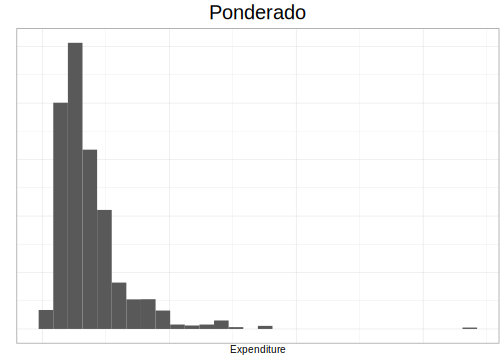
\includegraphics[keepaspectratio]{04-Continuas_files/figure-latex/hist2-1.pdf}}

Uno de los análisis gráficos más comunes que se realizan ene encuestas de hogares están relacionados con subgrupos geográficos como lo son las zonas (urbano - rural) o también realizar desagregaciones temáticas como lo son por sexo (hombre mujer). A continuación, se muestra la sintaxis en \texttt{R} como se realizan histogramas para hombres y mujeres mayores de 18 años:

\begin{Shaded}
\begin{Highlighting}[]
\NormalTok{sub\_Mujer  }\OtherTok{\textless{}{-}}\NormalTok{ diseno }\SpecialCharTok{\%\textgreater{}\%}  \FunctionTok{filter}\NormalTok{(Sex }\SpecialCharTok{==} \StringTok{"Female"}\NormalTok{)}
\NormalTok{sub\_Hombre }\OtherTok{\textless{}{-}}\NormalTok{ diseno }\SpecialCharTok{\%\textgreater{}\%}  \FunctionTok{filter}\NormalTok{(Sex }\SpecialCharTok{==} \StringTok{"Male"}\NormalTok{)}

\FunctionTok{par}\NormalTok{(}\AttributeTok{mfrow =} \FunctionTok{c}\NormalTok{(}\DecValTok{1}\NormalTok{,}\DecValTok{2}\NormalTok{))}

\FunctionTok{svyhist}\NormalTok{(}
  \SpecialCharTok{\textasciitilde{}}\NormalTok{ Income ,}
  \AttributeTok{design =} \FunctionTok{subset}\NormalTok{(sub\_Mujer, Age }\SpecialCharTok{\textgreater{}=} \DecValTok{18}\NormalTok{),}
  \AttributeTok{main =} \StringTok{"Mujer"}\NormalTok{,}
  \AttributeTok{breaks =} \DecValTok{30}\NormalTok{,}
  \AttributeTok{col =} \StringTok{"grey80"}\NormalTok{,}
  \AttributeTok{xlab =} \StringTok{"Ingreso"}\NormalTok{)}

\FunctionTok{svyhist}\NormalTok{(}
  \SpecialCharTok{\textasciitilde{}}\NormalTok{ Income ,}
  \AttributeTok{design =} \FunctionTok{subset}\NormalTok{(sub\_Hombre, Age }\SpecialCharTok{\textgreater{}=} \DecValTok{18}\NormalTok{),}
  \AttributeTok{main =} \StringTok{"Hombre"}\NormalTok{,}
  \AttributeTok{breaks =} \DecValTok{30}\NormalTok{,}
  \AttributeTok{col =} \StringTok{"grey80"}\NormalTok{,}
  \AttributeTok{xlab =} \StringTok{"Ingreso"}\NormalTok{)}
\end{Highlighting}
\end{Shaded}

\pandocbounded{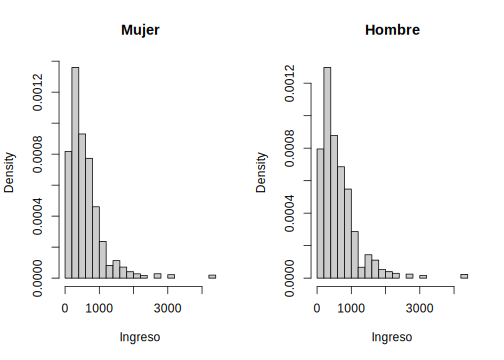
\includegraphics[keepaspectratio]{04-Continuas_files/figure-latex/unnamed-chunk-3-1.pdf}}

Como se puede observar, los argumentos utilizando para realizar los gráficos son los mismo que se utilizaron y ejemplificaron anteriormente. Cabe notar que la función \emph{subset} permite hacer un subconjunto de la población, que para nuetro caso son aquellos hombres y mujeres mayores o iguales a 18 años.

Si el objetivo ahora es realizar análisis de localización y variablidad, por ejemplo, graficar Bloxplot teniendo en cuenta los factores de expansión, a continuación, se muestran las sintaxis de como realizarlo en \texttt{R}.

\begin{Shaded}
\begin{Highlighting}[]
\NormalTok{sub\_Urbano }\OtherTok{\textless{}{-}}\NormalTok{ diseno }\SpecialCharTok{\%\textgreater{}\%}  \FunctionTok{filter}\NormalTok{(Zone }\SpecialCharTok{==} \StringTok{"Urban"}\NormalTok{)}
\NormalTok{sub\_Rural  }\OtherTok{\textless{}{-}}\NormalTok{ diseno }\SpecialCharTok{\%\textgreater{}\%}  \FunctionTok{filter}\NormalTok{(Zone }\SpecialCharTok{==} \StringTok{"Rural"}\NormalTok{)}

\FunctionTok{par}\NormalTok{(}\AttributeTok{mfrow =} \FunctionTok{c}\NormalTok{(}\DecValTok{1}\NormalTok{,}\DecValTok{2}\NormalTok{))}
\FunctionTok{svyboxplot}\NormalTok{(}
\NormalTok{  Income}\SpecialCharTok{\textasciitilde{}}\DecValTok{1}\NormalTok{ ,}
\NormalTok{  sub\_Urbano,}
  \AttributeTok{col =} \StringTok{"grey80"}\NormalTok{,}
  \AttributeTok{ylab =} \StringTok{"Ingreso"}\NormalTok{,}
  \AttributeTok{xlab =} \StringTok{"Urbano"}\NormalTok{)}

\FunctionTok{svyboxplot}\NormalTok{(}
\NormalTok{  Income }\SpecialCharTok{\textasciitilde{}} \DecValTok{1}\NormalTok{ ,}
\NormalTok{  sub\_Rural,}
  \AttributeTok{col =} \StringTok{"grey80"}\NormalTok{,}
  \AttributeTok{ylab =} \StringTok{"Ingreso"}\NormalTok{,}
  \AttributeTok{xlab =} \StringTok{"Rural"}\NormalTok{)}
\end{Highlighting}
\end{Shaded}

\pandocbounded{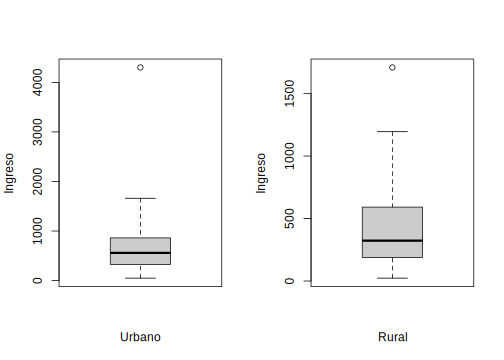
\includegraphics[keepaspectratio]{04-Continuas_files/figure-latex/box1-1.pdf}}

Los argumentos usados en la función \emph{svyboxplot} para generar el gráfico son muy similares a los usados en la función \emph{svyhist}. Algo a recalcar el los argumentos de esta función es que el símbolo ``Income \textasciitilde{} 1'' hace referencia a que todas las personas pertenecen a un solo grupo que puede ser urbano o rural dependiendo del caso y por eso se requiere indicarle a \texttt{R} esa restricción, lo cual se hace con el símbolo ``\textasciitilde1''.

\section{Estimación de totales, medias y razones}\label{estimaciuxf3n-de-totales-medias-y-razones}

Al trabajar con encuestas de hogares, el análisis de datos numéricos implica con frecuencia calcular estadísticas descriptivas como medias, totales y razones, ya que estas permiten sintetizar las principales características de la población y sirven de base para la toma de decisiones. Dichas estimaciones pueden calcularse para la población en su conjunto o para subgrupos específicos, según los objetivos de la investigación. Tal como destacan Heeringa, West y Berglund (2017), el cálculo de totales y medias poblacionales, junto con sus varianzas, ha sido esencial para el desarrollo de la teoría del muestreo probabilístico y la interpretación adecuada de los resultados de encuestas de hogares.

\subsection{Estimación puntual}\label{estimaciuxf3n-puntual}

Una vez exploradas las tendencias de las variables continuas mediante análisis gráfico, el siguiente paso consiste en obtener las estimaciones puntuales de los parámetros medidos. Estas estimaciones pueden calcularse de forma general o desagregada por niveles de análisis, dependiendo de las necesidades de la investigación. En el contexto de encuestas de hogares, las estimaciones puntuales comprenden el cálculo de totales, promedios, razones y otras medidas agregadas.

Heeringa et al.~(2017) señalan que la estimación del total o promedio de una población y su varianza muestral es fundamental en la teoría del muestreo probabilístico, ya que permite obtener valores precisos sobre la situación de los hogares estudiados, facilitando la toma de decisiones informadas en políticas públicas.

\subsection{Estimación de totales e intervalos de confianza}\label{estimaciuxf3n-de-totales-e-intervalos-de-confianza}

Una vez definido el diseño muestral (como se hizo en la sección anterior), se procede a realizar los procesos de estimación de los parámetros de interés. Para efectos de este texto, se iniciará con la estimación del total de los ingresos de los hogares.

En su mayoría, los paquetes estadísticos actuales no implementan técnicas avanzadas como estimadores generales de regresión (GREG) o métodos de calibración. Sin embargo, Valliant et al.~(2000) desarrollaron una librería en \emph{S-plus} que permite realizar estos procedimientos de estimación, los cuales también pueden implementarse en R (Valliant et al., 2013).

Para la estimación de totales con diseños muestrales complejos que incluyen estratificación (\(h=1,2,...,H\)) y muestreo por conglomerados (cuyos conglomerados están dentro del estrato \(h\), indexados por \(\alpha=1,2,...,a\_h\)), el estimador del total se puede expresar como:

\[
\hat{Y}_{\omega} = \sum_{h=1}^{H}\sum_{\alpha=1}^{a_h}\sum_{i=1}^{n_{h\alpha}}\omega_{h\alpha i} y_{h\alpha i}
\]

El estimador insesgado de la varianza para este total es:

\[
\text{var}\left(\hat{Y}_{\omega}\right) = \sum_{h=1}^{H} \frac{a_h}{a_h - 1} \left[ \sum_{\alpha=1}^{a_h} \left( \sum_{i=1}^{n_{h\alpha}} \omega_{h\alpha i} y_{h\alpha i} \right)^2 - \frac{\left( \sum_{\alpha=1}^{a_h} \omega_{h\alpha i} y_{h\alpha i} \right)^2}{a_h} \right]
\]

La determinación de los totales poblacionales constituye uno de los pilares del análisis de encuestas. Tanto las medias como las proporciones y las razones derivan de los totales. Un total se define como la suma de una variable específica (por ejemplo, ingreso o gasto) a nivel de toda la población. Para estimar el ingreso total de todos los hogares de un país, se combinan los datos de la muestra aplicando los pesos muestrales que reflejan el diseño y aseguran representatividad.

En el caso de variables numéricas simples, las estimaciones básicas son los totales y medias, mientras que las razones permiten establecer comparaciones entre dos variables numéricas. Estos cálculos pueden realizarse para toda la población o de manera desagregada por dominios de estudio, dependiendo de las preguntas de investigación.

Para encuestas con estratificación (\(h=1,2,...,H\)) y submuestreo en las UPM (ubicadas dentro de cada estrato \(h\), identificadas por \(i\)), el total poblacional se estima mediante:

\[
\hat{Y} = \sum_{h=1}^{H} \sum_{i \in s_{1h}} \sum_{k \in s_{hi}} w_{hik} \, y_{hik}
\]

Cuando se cuenta con respuesta completa, la varianza de \(\hat{Y}\) puede calcularse usando el estimador de Ultimate Cluster.

El intervalo de confianza de nivel \(1-\alpha\) para el total poblacional \(Y\) se calcula como:

\[
\hat{Y} \pm t_{1-\alpha/2, df} \times \sqrt{\hat{V}_{UC}(\hat{Y})}
\]

A medida que los grados de libertad aumentan, la distribución \(t\) de Student tiende a la normal, lo que explica por qué muchas Oficinas Nacionales de Estadística (ONE) utilizan esta aproximación para reportar intervalos de confianza. No obstante, es importante considerar que esta aproximación puede ser menos fiable cuando el tamaño de la muestra es reducido, aunque suele ofrecer buenos resultados en encuestas de hogares extensas.

Como se puede observar, calcular la estimación del total y su varianza estimada es complejo.

\subsubsection{Enfoques para la estimación de la varianza}\label{enfoques-para-la-estimaciuxf3n-de-la-varianza}

Tal como se mencionó anteriormente, al trabajar con encuestas de hogares es fundamental proporcionar no solo estimaciones puntuales, sino también cuantificar la incertidumbre asociada a dichas estimaciones. Comprender y estimar esta incertidumbre constituye una parte crítica del análisis de los datos provenientes de encuestas de hogares. Mediante la aplicación de métodos apropiados, los usuarios pueden medir la precisión de sus estimaciones.

Existen diversos métodos para estimar dicha precisión y, con el apoyo de software moderno, estos enfoques pueden implementarse de manera eficiente para respaldar análisis rigurosos y significativos. Entre los principales métodos se encuentran:

\begin{itemize}
\item
  \textbf{Ecuaciones de estimación:} ofrecen un marco flexible para estimar totales, medias, razones y otros parámetros, así como sus varianzas correspondientes, integrando una idea unificadora de la teoría de muestreo (Binder, 1983).
\item
  \textbf{Linealización de Taylor:} consiste en aproximar estadísticas no lineales complejas mediante expresiones lineales y posteriormente estimar la varianza de esta cantidad aproximada.
\item
  \textbf{Método del Clúster Último:} utilizado con frecuencia en encuestas que emplean muestreo estratificado en múltiples etapas; se basa en calcular la varianza a partir de las diferencias entre las estimaciones obtenidas a nivel de las unidades primarias de muestreo (PSU). Suele combinarse con la Linealización de Taylor para estimar la varianza de estadísticas no lineales, como medias o razones.
\item
  \textbf{Bootstrap y otros métodos de replicación:} se fundamentan en tomar repetidas submuestras del conjunto de datos observado, calcular estimaciones para cada réplica y luego utilizar la variabilidad entre estas estimaciones replicadas para inferir la varianza del estimador principal.
\end{itemize}

\subsubsection*{Ecuaciones de estimación y linealización de Taylor}\label{ecuaciones-de-estimaciuxf3n-y-linealizaciuxf3n-de-taylor}
\addcontentsline{toc}{subsubsection}{Ecuaciones de estimación y linealización de Taylor}

Como se mencionó en el apartado anterior, uno de los enfoques más utilizados para cuantificar la incertidumbre en encuestas de hogares se basa en la formulación de \textbf{ecuaciones de estimación} y en la aplicación de la \textbf{linealización de Taylor}. Estos métodos proporcionan un marco general que permite definir los parámetros de interés, obtener sus estimadores muestrales y, a partir de ellos, aproximar sus varianzas.

Muchos parámetros poblacionales pueden expresarse como soluciones de ecuaciones de estimación que involucran totales poblacionales. Aunque los detalles técnicos pueden ser complejos, la idea fundamental es que los mismos principios utilizados para estimar totales pueden aplicarse también para la estimación de varianzas. Este marco general hace que el método sea sencillo y versátil, permitiendo una implementación eficiente en software especializado.

Una ecuación de estimación poblacional genérica se expresa como:

\[
\sum_{k\in U} z_k(\theta)=0,
\]

donde \(z_k(\cdot)\) es una función de estimación evaluada para la unidad \(k\) y \(\theta\) representa el parámetro poblacional de interés. Estas ecuaciones proporcionan un marco general para definir y calcular diversos parámetros de la población, como totales, medias y razones.

\begin{itemize}
\item
  \textbf{Para el total poblacional:}
  \(z_k(\theta)=y_k-\theta/N\). La ecuación de estimación es \(\sum_{k\in U}(y_k-\theta/N)=0\), cuya solución es \(\theta=\sum_{k\in U} y_k = Y\).
\item
  \textbf{Para la media poblacional:}
  \(z_k(\theta)=y_k-\theta\). La ecuación es \(\sum_{k\in U}(y_k-\theta)=0\), cuya solución es \(\theta=\left(\sum_{k\in U} y_k\right)/N = \overline{Y}\).
\item
  \textbf{Para razones de totales:}
  \(z_k(\theta)=y_k-\theta x_k\). La ecuación \(\sum_{k\in U}(y_k-\theta x_k)=0\) conduce a la razón poblacional \(\theta=\dfrac{\sum_{k\in U} y_k}{\sum_{k\in U} x_k} = R\).
\end{itemize}

La idea de definir parámetros poblacionales como soluciones de ecuaciones de estimación a nivel de población conduce naturalmente a un método general para obtener los \textbf{estimadores muestrales}. En este caso, se utilizan ecuaciones de la forma:

\[
\sum_{k\in s} d_k\, z_k(\theta)=0,
\]

donde \(d_k\) son los pesos de diseño y \(z_k(\theta)\) la función de estimación evaluada para cada unidad de la muestra. Bajo un muestreo probabilístico y asumiendo respuesta completa, la suma muestral \(\sum_{k\in s} d_k\, z_k(\theta)\) es insesgada respecto a su análoga poblacional, lo que garantiza que las soluciones de estas ecuaciones sean estimadores consistentes de los parámetros poblacionales.

La \textbf{linealización de Taylor} constituye un complemento natural a este marco, ya que permite aproximar la varianza de estimadores no lineales. El procedimiento consiste en aplicar una expansión de Taylor de primer orden alrededor del parámetro estimado, con el fin de reemplazar el estimador no lineal por una expresión lineal. De esta manera, se facilita el cálculo de varianzas en situaciones donde no existen fórmulas exactas o su derivación resulta demasiado compleja.

Un estimador consistente de la varianza, derivado mediante linealización de Taylor para soluciones de ecuaciones de estimación muestrales, puede expresarse como:

\[
\hat{V}_{TL}(\hat{\theta}) = [\hat{J}(\hat{\theta})]^{-1} \, \hat{V}_p \Bigg[\sum_{k\in s} d_k\, z_k(\hat{\theta})\Bigg] \, [\hat{J}(\hat{\theta})]^{-1}
\]

donde \(\hat{J}(\hat{\theta}) = \sum_{k\in s} d_k \left[ \frac{\partial z_k(\theta)}{\partial \theta} \right]_{\theta=\hat{\theta}}\).

Este resultado muestra cómo la linealización de Taylor convierte la estimación de varianzas de parámetros complejos en un problema de estimación de totales, lo que explica su amplia adopción en software especializado para el análisis de encuestas.

\subsubsection*{Ultimate Cluster}\label{ultimate-cluster}
\addcontentsline{toc}{subsubsection}{Ultimate Cluster}

El método del Ultimate Cluster constituye un enfoque directo y robusto para estimar la varianza de totales en encuestas que emplean diseños de muestreo por conglomerados estratificados en múltiples etapas. Propuesto por Hansen, Hurwitz y Madow (1953), este método simplifica la complejidad de los diseños multinivel al centrarse únicamente en la variación entre las Unidades Primarias de Muestreo (PSU). Se asume que, dentro de cada estrato de muestreo, las PSU fueron seleccionadas de manera independiente con reemplazo (posiblemente con probabilidades desiguales), aunque en la práctica la selección suele realizarse sin reemplazo.

El método se basa en la variación entre las estadísticas calculadas a nivel de PSU. Cuando se aplica correctamente, refleja implícitamente cualquier submuestreo realizado dentro de las PSU, permitiendo estimaciones de varianza más simples pero confiables. Es especialmente útil en diseños complejos que incluyen estratificación y probabilidades desiguales de selección tanto de PSU como de unidades de niveles inferiores (hogares e individuos).

Los requisitos para aplicar este método son:

\begin{itemize}
\tightlist
\item
  Disponibilidad de estimaciones insesgadas de totales para las variables de interés en cada PSU muestreada.
\item
  Al menos dos PSU muestreadas por estrato, si la muestra se estratifica en la primera etapa.
\item
  Información completa sobre PSU, estratos y pesos en el conjunto de datos de la encuesta.
\end{itemize}

Considere un diseño de muestreo en múltiples etapas donde se seleccionan \(n_h\) PSU en el estrato \(h\), \(h=1,\dots,H\). Sea

\[
\hat{Y}_{hi} = \sum_{k\in s_{hi}} d_{hik} y_{hik}
\]

una estimación del total poblacional \(Y_{hi}\) de la PSU \(i\) en el estrato \(h\). Un estimador insesgado del total poblacional \(Y = \sum_{h=1}^H \sum_{i \in U_{1h}} Y_{hi}\) se expresa como

\[
\hat{Y}_{UC} = \sum_{h=1}^H \hat{Y}_h, \quad \text{donde} \quad \hat{Y}_h = \frac{1}{n_h} \sum_{i\in s_{1h}} \hat{Y}_{hi}.
\]

El estimador Ultimate Cluster de la varianza correspondiente se calcula mediante:

\[
\hat{V}_{UC}(\hat{Y}) = \sum_{h=1}^H \frac{n_h}{n_h-1} \sum_{i \in s_{1h}} (\hat{Y}_{hi} - \hat{Y}_h)^2
\]

Para más detalles, véase Hansen, Hurwitz y Madow (1953, vol.~I, p.~257) o Wolter (2007).

Aunque originalmente se diseñó para calcular varianzas de estimadores de totales, el método puede combinarse con linealización de Taylor o ecuaciones de estimación para derivar varianzas de otros parámetros poblacionales formulables como soluciones de ecuaciones de estimación. Esta flexibilidad hace que el método sea aplicable a diversos contextos de análisis de encuestas de hogares.

Un supuesto clave es que, dentro de cada estrato, las PSU se eligen de forma independiente y con reemplazo. En la práctica, la mayoría de las encuestas selecciona PSU sin reemplazo, generando diseños más eficientes. Así, las varianzas calculadas bajo la hipótesis de independencia constituyen aproximaciones de las verdaderas varianzas de muestreo. Cuando la fracción muestral es pequeña (por ejemplo, \textless5\,\%), estas aproximaciones suelen ser suficientemente precisas para su uso por oficinas nacionales de estadística o analistas secundarios.

El método Ultimate Cluster destaca por su simplicidad y robustez, lo que lo hace muy atractivo en la práctica. Aunque los métodos más sofisticados que consideran todas las etapas del diseño pueden ofrecer estimaciones de varianza ligeramente más precisas, su aplicación requiere información más detallada y mayor complejidad computacional. Por el contrario, el método Ultimate Cluster proporciona una aproximación confiable y eficiente, especialmente útil al estimar totales o medias en encuestas de hogares. Para un análisis detallado sobre la precisión de esta aproximación y posibles alternativas, véase Särndal, Swensson y Wretman (1992, p.~153).

\subsubsection*{Bootstrap}\label{bootstrap}
\addcontentsline{toc}{subsubsection}{Bootstrap}

En muchos casos, los microdatos de encuestas públicas omiten información esencial del diseño, como identificadores de estratos o de unidades primarias de muestreo (UPM), para proteger la confidencialidad de los encuestados. Esta omisión limita la capacidad de los usuarios para calcular varianzas válidas. En tales situaciones, se recomienda que las oficinas nacionales de estadística (NSO) proporcionen pesos de replicación, lo que permite a los analistas estimar errores estándar de manera correcta. Sin estos datos, los usuarios secundarios no pueden reproducir los errores estándar publicados ni considerar adecuadamente el diseño complejo de la encuesta.

Los métodos de replicación estiman la varianza generando subconjuntos de la muestra original, calculando estimaciones para cada uno y utilizando la variabilidad observada entre estas estimaciones para aproximar la varianza del estimador principal. Son particularmente útiles cuando no se dispone de información sobre estratos o UPM, situación en la que no se puede aplicar el método de Ultimate Cluster.

El Bootstrap es una herramienta de replicación robusta y versátil. Originalmente introducido por Efron (1979) para datos que no provenían de encuestas, su adaptación más usada para encuestas de hogares es el Bootstrap de Reescalamiento Rao-Wu-Yue (Rao, Wu y Yue, 1992). Este método se ajusta de manera óptima a diseños de muestreo estratificados y multietápicos, y es ampliamente empleado para la estimación de varianzas en encuestas complejas.

El procedimiento consiste en generar muchas réplicas de la muestra original, simulando extracciones repetidas de la población. Cada réplica se construye mediante la creación de columnas adicionales de pesos de replicación en la base de datos, siguiendo este proceso:

\begin{itemize}
\tightlist
\item
  Para cada estrato, se seleccionan aleatoriamente las UPM con reemplazo; algunas pueden repetirse y otras no aparecer. Cada UPM elegida se incorpora con todas sus observaciones. Si el tamaño de la muestra de primera etapa en el estrato \(h\) es mayor que dos (\(n_h > 2\)), el número de UPM seleccionadas por réplica es \(n_h - 1\).
\item
  Este proceso se repite muchas veces, habitualmente cientos, generando un gran número de réplicas. La cantidad de veces que una UPM \(i\) del estrato \(h\) aparece en la réplica \(r\) se denota \(n_{hi}^{(r)}\), variando entre 0 y \(n_h - 1\).
\item
  A partir de cada réplica se calculan nuevos pesos bootstrap para todas las unidades, reflejando cuántas veces fue seleccionada su UPM. El peso de la unidad \(k\) en la réplica \(r\) se calcula como:
\end{itemize}

\[
w_{hik}^{(r)} = w_{hik} \times \frac{n_h}{n_h - 1} \times n_{hi}^{(r)}
\]

Si los pesos originales incluyen ajustes por no respuesta o calibración, estos deben aplicarse también a cada conjunto de pesos bootstrap.

Cuando la NSO proporciona únicamente pesos de replicación Bootstrap, los analistas pueden estimar errores estándar correctamente, aun sin identificadores de estratos o UPM. Para cada réplica \(r\), se calcula el parámetro de interés \(\hat{\theta}^{(r)}\) usando los pesos bootstrap \(w_{hik}^{(r)}\). La varianza del estimador original se aproxima mediante la variabilidad entre todas las réplicas:

\[
\hat{V}_B(\hat{\theta}) = \frac{1}{R} \sum_{r=1}^{R} \left(\hat{\theta}^{(r)} - \tilde{\theta}\right)^2, \quad
\tilde{\theta} = \frac{1}{R} \sum_{r=1}^{R} \hat{\theta}^{(r)}
\]

Este enfoque asegura que la dispersión entre réplicas capture fielmente la incertidumbre del parámetro.

El Bootstrap ofrece múltiples ventajas. A pesar de requerir un mayor procesamiento computacional, es eficaz para diseños de encuesta complejos y permite estimar parámetros difíciles de calcular con métodos tradicionales, como medianas u otras estadísticas no lineales. Es especialmente útil para analistas que trabajan con bases de datos sin identificadores de estratos y UPM, pero con pesos de replicación.

La simplicidad del método facilita su aplicación incluso sin software estadístico especializado. Sin embargo, la mayoría de los paquetes estadísticos modernos ya incluyen procedimientos para aplicar Bootstrap y calcular varianzas, ampliando su disponibilidad y robustez. No obstante, su uso no es recomendable en encuestas repetidas con muestras superpuestas ni en situaciones con fracciones de muestreo grandes y tamaños de muestra pequeños (Bruch, 2011).

En este ejemplo se muestra cómo estimar totales y sus intervalos de confianza para diferentes variables de interés en R, utilizando dos funciones de la librería survey: la función svytotal para calcular los totales y la función confint para obtener los intervalos de confianza. A continuación, se presentan los códigos correspondientes:

\begin{Shaded}
\begin{Highlighting}[]
\NormalTok{total\_Ingresos}\OtherTok{\textless{}{-}} \FunctionTok{svytotal}\NormalTok{(}\SpecialCharTok{\textasciitilde{}}\NormalTok{Income, diseno, }\AttributeTok{deff=}\NormalTok{T, )}
\NormalTok{total\_Ingresos}
\end{Highlighting}
\end{Shaded}

\begin{verbatim}
##           total       SE DEff
## Income 85793667  4778675   11
\end{verbatim}

\begin{Shaded}
\begin{Highlighting}[]
\FunctionTok{confint}\NormalTok{(total\_Ingresos, }\AttributeTok{level =} \FloatTok{0.95}\NormalTok{)}
\end{Highlighting}
\end{Shaded}

\begin{verbatim}
##           2.5 %   97.5 %
## Income 76427637 95159697
\end{verbatim}

Los argumentos que utiliza de la función \texttt{svytotal} con muy sencillos. Para el ejemplo, se le introduce primero la variable en la cual está la información que se desea estimar (Income). Posterior a esto, se introduce el diseño muestral del cual proviene la muestra y, por último, se indica si desea que se reporte el deff de la estimación o no.

Por otro lado, para el cálculo del intervalo de confianza, lo único que requiere es indicarle a la función \texttt{confint} el estimador y la confianza requerida.

Paras seguir ilustrando el uso de la función \texttt{svytotal} y de \texttt{confint}, estimemos el total de gastos de los hogares, pero ahora el intervalo de confianza se calculará al 90\% de confianza. Los siguientes códigos realizan las estimaciones:

\begin{Shaded}
\begin{Highlighting}[]
\NormalTok{total\_gastos}\OtherTok{\textless{}{-}} \FunctionTok{svytotal}\NormalTok{ (}\SpecialCharTok{\textasciitilde{}}\NormalTok{Expenditure, diseno, }\AttributeTok{deff=}\NormalTok{T)}
\NormalTok{total\_gastos}
\end{Highlighting}
\end{Shaded}

\begin{verbatim}
##                total       SE   DEff
## Expenditure 55677504  2604139 10.222
\end{verbatim}

\begin{Shaded}
\begin{Highlighting}[]
\FunctionTok{confint}\NormalTok{(total\_gastos, }\AttributeTok{level =} \FloatTok{0.9}\NormalTok{)}
\end{Highlighting}
\end{Shaded}

\begin{verbatim}
##                  5 %     95 %
## Expenditure 51394077 59960931
\end{verbatim}

Si el objetivo ahora es estimar el total de los ingreso de los hogares pero discriminado por sexo, se utilizará ahora la función \texttt{cascade}de la libraría \texttt{srvyr}, la cual permite agregar
la suma de las categorías al final la tabla. También se utilizará la función \texttt{group\_by} la cual permite obtener resultados agrupados por los niveles de interés.

\begin{Shaded}
\begin{Highlighting}[]
\NormalTok{diseno }\SpecialCharTok{\%\textgreater{}\%} \FunctionTok{group\_by}\NormalTok{(Sex) }\SpecialCharTok{\%\textgreater{}\%}
  \FunctionTok{cascade}\NormalTok{(}\AttributeTok{Total =} \FunctionTok{survey\_total}\NormalTok{(}
\NormalTok{    Income, }\AttributeTok{level =} \FloatTok{0.95}\NormalTok{,}
    \AttributeTok{vartype =}  \FunctionTok{c}\NormalTok{(}\StringTok{"se"}\NormalTok{, }\StringTok{"ci"}\NormalTok{)),}
          \AttributeTok{.fill =} \StringTok{"Total ingreso"}\NormalTok{)}
\end{Highlighting}
\end{Shaded}

\begin{verbatim}
## # A tibble: 3 x 5
##   Sex               Total Total_se Total_low Total_upp
##   <chr>             <dbl>    <dbl>     <dbl>     <dbl>
## 1 Female        44153820. 2324452. 39551172. 48756467.
## 2 Male          41639847. 2870194. 35956576. 47323118.
## 3 Total ingreso 85793667. 4778674. 76331414. 95255920.
\end{verbatim}

Como se pudo observar en lo códigos anteriores, otra forma de obtener las estimaciones del total, su desviación estándar y el intervalo de confianza es usando el argumento \texttt{vartype} e indicándole las opciones ``se'', ``ci'' respectivamente.

\subsection{Estimación de la media e intervalo de confianza}\label{estimaciuxf3n-de-la-media-e-intervalo-de-confianza}

La estimación de la media poblacional es un parámetro muy importante en las encuestas de hogares, dado que, por ejemplo, uno de los indicadores trazadores en este tipo de encuestas son los ingresos medios por hogar. Además, este tipo de parámetros no permiten describir y analizar las tendencias centrales de estas variables en poblaciones de interés. Según \textbf{Gutiérrez (2016)} un estimador de la media poblacional se puede escribir como una razón no lineal de dos totales de población finitas estimados como sigue:

\begin{eqnarray*}
\bar{Y}_{\omega} & = & \frac{\sum_{h=1}^{H}\sum_{\alpha=1}^{a_{h}}\sum_{i=1}^{n_{h\alpha}}\omega_{h\alpha i}y_{h\alpha i}}{\sum_{h=1}^{H}\sum_{\alpha=1}^{a_{h}}\sum_{i=1}^{n_{h\alpha}}\omega_{h\alpha i}}\\
 & = & \frac{\hat{Y}}{\hat{N}}.
\end{eqnarray*}

Como una observación tenga en cuenta que, si \(y\) es una variable
binaria, la media ponderada estima la proporción de la población.
Por otro lado, como \(\bar{Y}_{\omega}\) no es una estadística lineal,
no existe una fórmula cerrada para la varianza de este estimador.
Es por lo anterior que, se deben recurrir a usar métodos de remuestreo
o series de Taylor. Para este caso en particular, usando series de
Taylor el estimador insesgado de la varianza para este estimador es:

\begin{eqnarray*}
var\left(\bar{Y}_{\omega}\right) & \dot{=} & \frac{var\left(\hat{Y}\right)+\bar{Y}_{\omega}^{2}\times var\left(\hat{N}\right)-2\times\bar{Y}_{\omega}\times cov\left(\hat{Y},\hat{N}\right)}{\hat{N}^{2}}
\end{eqnarray*}

Como se puede observar, el cálculo de la estimación de la varianza tiene componentes complejos de calcular de manera analítica, como la covarianza entre el total estimado y el tamaño poblacional estimado. Sin embargo, \texttt{R} tiene funciones que incorpora estos estimadores. A continuación, se presenta la sintaxis para hacer dichos cálculos.

\begin{Shaded}
\begin{Highlighting}[]
\NormalTok{Media\_ingresos}\OtherTok{\textless{}{-}} \FunctionTok{svymean}\NormalTok{(}\SpecialCharTok{\textasciitilde{}}\NormalTok{Income, diseno, }\AttributeTok{deff=}\NormalTok{T)}
\NormalTok{Media\_ingresos}
\end{Highlighting}
\end{Shaded}

\begin{verbatim}
##           mean      SE   DEff
## Income 570.945  28.478 8.8211
\end{verbatim}

\begin{Shaded}
\begin{Highlighting}[]
\FunctionTok{confint}\NormalTok{(Media\_ingresos, }\AttributeTok{level =} \FloatTok{0.95}\NormalTok{)}
\end{Highlighting}
\end{Shaded}

\begin{verbatim}
##           2.5 %   97.5 %
## Income 515.1299 626.7607
\end{verbatim}

Como se puede observar, los argumentos que utiliza la función \texttt{svymean} para realizar la estimación de la media de los ingresos de los hogares y la desviación estándar estimada del estimador son similares a los utilizando con la función \texttt{svytotal}. Similarmente ocurre con el intervalo de confianza.

Por otro lado, tal como se realizó con el total, a manera de ejemplo, se estima la media de los gastos en los hogares como sigue a continuación:

\begin{Shaded}
\begin{Highlighting}[]
\NormalTok{Media\_gastos}\OtherTok{\textless{}{-}} \FunctionTok{svymean}\NormalTok{ (}\SpecialCharTok{\textasciitilde{}}\NormalTok{Expenditure, diseno, }\AttributeTok{deff=}\NormalTok{T)}
\NormalTok{Media\_gastos}
\end{Highlighting}
\end{Shaded}

\begin{verbatim}
##                mean      SE   DEff
## Expenditure 370.526  13.294 6.0156
\end{verbatim}

\begin{Shaded}
\begin{Highlighting}[]
\FunctionTok{confint}\NormalTok{(Media\_gastos)}
\end{Highlighting}
\end{Shaded}

\begin{verbatim}
##                2.5 %   97.5 %
## Expenditure 344.4697 396.5829
\end{verbatim}

También se pueden realizar estimaciones de la media por subgrupos siguiendo el mismo esquema mostrado para la función \texttt{svytotal}. Particularmente, los gastos de los hogares discriminados por sexo es:

\begin{Shaded}
\begin{Highlighting}[]
\NormalTok{diseno }\SpecialCharTok{\%\textgreater{}\%} \FunctionTok{group\_by}\NormalTok{(Sex) }\SpecialCharTok{\%\textgreater{}\%}
  \FunctionTok{cascade}\NormalTok{(}
    \AttributeTok{Media =} \FunctionTok{survey\_mean}\NormalTok{(}
\NormalTok{      Expenditure, }\AttributeTok{level =} \FloatTok{0.95}\NormalTok{,}
       \AttributeTok{vartype =}  \FunctionTok{c}\NormalTok{(}\StringTok{"se"}\NormalTok{, }\StringTok{"ci"}\NormalTok{)),}
        \AttributeTok{.fill =} \StringTok{"El gasto medio"}\NormalTok{  ) }\SpecialCharTok{\%\textgreater{}\%}
  \FunctionTok{arrange}\NormalTok{(}\FunctionTok{desc}\NormalTok{(Sex))}
\end{Highlighting}
\end{Shaded}

\begin{verbatim}
## # A tibble: 3 x 5
##   Sex            Media Media_se Media_low Media_upp
##   <chr>          <dbl>    <dbl>     <dbl>     <dbl>
## 1 Male            374.     16.1      343.      406.
## 2 Female          367.     12.3      343.      391.
## 3 El gasto medio  371.     13.3      344.      397.
\end{verbatim}

Por zona,

\begin{Shaded}
\begin{Highlighting}[]
\NormalTok{diseno }\SpecialCharTok{\%\textgreater{}\%} \FunctionTok{group\_by}\NormalTok{(Zone) }\SpecialCharTok{\%\textgreater{}\%}
  \FunctionTok{cascade}\NormalTok{(}
    \AttributeTok{Media =} \FunctionTok{survey\_mean}\NormalTok{(}
\NormalTok{      Expenditure, }\AttributeTok{level =} \FloatTok{0.95}\NormalTok{,}
       \AttributeTok{vartype =}  \FunctionTok{c}\NormalTok{(}\StringTok{"se"}\NormalTok{, }\StringTok{"ci"}\NormalTok{)),}
        \AttributeTok{.fill =} \StringTok{"El gasto medio"}\NormalTok{)}\SpecialCharTok{\%\textgreater{}\%}
  \FunctionTok{arrange}\NormalTok{(}\FunctionTok{desc}\NormalTok{(Zone))}
\end{Highlighting}
\end{Shaded}

\begin{verbatim}
## # A tibble: 3 x 5
##   Zone           Media Media_se Media_low Media_upp
##   <chr>          <dbl>    <dbl>     <dbl>     <dbl>
## 1 Urban           460.     22.2      416.      504.
## 2 Rural           274.     10.3      254.      294.
## 3 El gasto medio  371.     13.3      344.      397.
\end{verbatim}

Por sexo y zona,

\begin{Shaded}
\begin{Highlighting}[]
\NormalTok{diseno }\SpecialCharTok{\%\textgreater{}\%} \FunctionTok{group\_by}\NormalTok{(Zone, Sex) }\SpecialCharTok{\%\textgreater{}\%}
  \FunctionTok{cascade}\NormalTok{(}
    \AttributeTok{Media =} \FunctionTok{survey\_mean}\NormalTok{(}
\NormalTok{      Expenditure, }\AttributeTok{level =} \FloatTok{0.95}\NormalTok{,}
       \AttributeTok{vartype =}  \FunctionTok{c}\NormalTok{(}\StringTok{"se"}\NormalTok{, }\StringTok{"ci"}\NormalTok{)),}
        \AttributeTok{.fill =} \StringTok{"El gasto medio"}\NormalTok{) }\SpecialCharTok{\%\textgreater{}\%}
  \FunctionTok{arrange}\NormalTok{(}\FunctionTok{desc}\NormalTok{(Zone), }\FunctionTok{desc}\NormalTok{(Sex)) }\SpecialCharTok{\%\textgreater{}\%}
  \FunctionTok{data.frame}\NormalTok{()}
\end{Highlighting}
\end{Shaded}

\begin{verbatim}
##             Zone            Sex    Media Media_se Media_low Media_upp
## 1          Urban           Male 469.8124 26.96068  416.4276  523.1973
## 2          Urban         Female 450.8151 20.11853  410.9784  490.6518
## 3          Urban El gasto medio 459.6162 22.20655  415.6450  503.5874
## 4          Rural           Male 275.3018 10.24848  255.0088  295.5948
## 5          Rural         Female 272.6769 11.61470  249.6786  295.6751
## 6          Rural El gasto medio 273.9461 10.26141  253.6275  294.2647
## 7 El gasto medio El gasto medio 370.5263 13.29444  344.2020  396.8506
\end{verbatim}

Las medias o promedios poblacionales son esenciales para describir la tendencia central de una variable. Por ejemplo, el gasto promedio de los hogares es un indicador representativo del comportamiento económico de la población. Su cálculo consiste en dividir el total estimado de la variable entre el tamaño poblacional estimado, de modo que su precisión depende de la exactitud en ambos componentes.

El estimador de la media poblacional se puede expresar como:

\[
\widehat{\bar{Y}} = \frac{\displaystyle \sum_{h=1}^{H} \sum_{i \in s_{1h}} \sum_{k \in s_{hi}} w_{hik} y_{hik}} {\displaystyle \sum_{h=1}^{H} \sum_{i \in s_{1h}} \sum_{k \in s_{hi}} w_{hik}} = \frac{\hat{Y}}{\hat{N}}
\]

Dado que \(\widehat{\bar{Y}}\) es un estimador no lineal, su varianza exacta no puede expresarse en forma cerrada. Por ello, los paquetes estadísticos especializados en encuestas complejas emplean métodos como el remuestreo o la aproximación de Taylor, que se implementan automáticamente para facilitar su cálculo.

\subsection{Estimación de medidas de dispersión y localización}\label{estimaciuxf3n-de-medidas-de-dispersiuxf3n-y-localizaciuxf3n}

En las encuestas de hogares siempre es necesario estimar medidas de dispersión de las variables estudiadas. Esto con el fin de, por ejemplo, ver qué tan disímiles son los ingresos medios de los hogares en un país determinado y con esto poder tomar acciones de política pública. Por lo anterior, es importante estudiar este parámetro en este texto. A continuación, se presenta el estimador de la desviación estándar:

\begin{eqnarray}
s\left(y\right){}_{\omega} & = & \frac{\sum_{h=1}^{H}\sum_{\alpha=1}^{a_{h}}\sum_{i=1}^{n_{h\alpha}}\omega_{h\alpha i}\left(y_{h\alpha i}-\bar{Y}_{\omega}\right)^{2}}{\sum_{h=1}^{H}\sum_{\alpha=1}^{a_{h}}\sum_{i=1}^{n_{h\alpha}}\omega_{h\alpha i}-1}
\end{eqnarray}

Para llevar a cabo la estimación en \texttt{R} de la desviación estándar en encuestas de hogares, se utilizan la función \texttt{survey\_var} la cual se ejemplifica a continuación:

\begin{Shaded}
\begin{Highlighting}[]
\NormalTok{(sd\_Est }\OtherTok{\textless{}{-}}\NormalTok{ diseno }\SpecialCharTok{\%\textgreater{}\%} \FunctionTok{group\_by}\NormalTok{(Zone) }\SpecialCharTok{\%\textgreater{}\%}
   \FunctionTok{summarise}\NormalTok{(}\AttributeTok{Sd =} \FunctionTok{sqrt}\NormalTok{(}
  \FunctionTok{survey\_var}\NormalTok{(}
\NormalTok{    Income,}
    \AttributeTok{level =} \FloatTok{0.95}\NormalTok{,}
    \AttributeTok{vartype =}  \FunctionTok{c}\NormalTok{(}\StringTok{"se"}\NormalTok{, }\StringTok{"ci"}\NormalTok{),}
\NormalTok{  ) )))}
\end{Highlighting}
\end{Shaded}

\begin{verbatim}
## # A tibble: 2 x 5
##   Zone     Sd Sd_se Sd_low Sd_upp
##   <chr> <dbl> <dbl>  <dbl>  <dbl>
## 1 Rural  310.  117.   263.   352.
## 2 Urban  582.  285.   422.   707.
\end{verbatim}

Como se pudo ver en el ejemplo anterior, se estimó la desviación estándar de los ingresos por zona reportando el error estándar en la estimación y un intervalo de confianza al 95\%. Los argumentos que utiliza la función \texttt{survey\_var} son similares a los usados en las funciones anteriores para estimar medias y totales.

Si el interés ahora se centra en estimar la desviación estándar clasificando por sexo y zona, los códigos computacionales son los siguientes:

\begin{Shaded}
\begin{Highlighting}[]
\NormalTok{(sd\_Est }\OtherTok{\textless{}{-}}\NormalTok{ diseno }\SpecialCharTok{\%\textgreater{}\%} \FunctionTok{group\_by}\NormalTok{(Zone, Sex) }\SpecialCharTok{\%\textgreater{}\%}
   \FunctionTok{summarise}\NormalTok{(}\AttributeTok{Sd =} \FunctionTok{sqrt}\NormalTok{(}
  \FunctionTok{survey\_var}\NormalTok{(}
\NormalTok{    Income,}
    \AttributeTok{level =} \FloatTok{0.95}\NormalTok{,}
    \AttributeTok{vartype =}  \FunctionTok{c}\NormalTok{(}\StringTok{"se"}\NormalTok{, }\StringTok{"ci"}\NormalTok{),}
\NormalTok{   )}
\NormalTok{))) }\SpecialCharTok{\%\textgreater{}\%} \FunctionTok{data.frame}\NormalTok{()}
\end{Highlighting}
\end{Shaded}

\begin{verbatim}
##    Zone    Sex       Sd    Sd_se   Sd_low   Sd_upp
## 1 Rural Female 294.8683 111.6203 249.5537 334.0921
## 2 Rural   Male 325.7584 124.9643 274.2209 370.1890
## 3 Urban Female 568.3920 286.4585 400.7312 696.8166
## 4 Urban   Male 596.7756 288.9435 436.8362 722.1194
\end{verbatim}

Las medidas de posición no central (Percentiles) se diseñaron con el fin de conocer otros puntos característicos de la distribución de los datos que no son los valores centrales. Entre las medidas de posición no central más importantes están la mediana, cuartiles y percentiles. En la mayoría de las encuestas de hogares no solo estiman totales, medias y proporciones. En algunos indicadores es necesario estimar otros parámetros, por ejemplo, medianas y percentiles. Como lo menciona \textbf{Tellez et al (2015)} la mediana una medida de tendencia central la cual, a diferencia del promedio, no es fácilmente influenciada por datos atípicos y, por esto, se conoce como una medida robusta. La mediana es el valor que divide la población en dos partes iguales. Lo que implica que, la mitad de las observaciones de la característica de interés está por encima de la media y la otra mitad está por debajo.

Por otro lado, la estimación de percentiles de ingresos en un país determinado puede definir el inicio de una política pública. por ejemplo, poner a tributar aquellas personas naturales que son el 10\% más alto de la distribución de los ingresos o por el contrario, generar subsidios de transporte a aquellas familias que están en el 15\% inferior de la distribución de los ingresos.

La estimación de cuantiles \textbf{(Loomis et al., 2005)} se basa en los resultados relacionados con el estimador ponderado para totales, empleando una estimación de la función de distribución (CDF, por sus siglas en inglés) acumulada de la población. Específicamente, la CDF para una variable y en una población finita dada de tamaño \(N\) se define de la siguiente manera:

\begin{eqnarray*}
F\left(x\right) & = & \frac{{ \sum_{i=1}^{N}}I\left(y_{i}\leq x\right)}{N}
\end{eqnarray*}

Donde, \(I\left(y_{i}\leq x\right)\) es una variable indicadora la
cual es igual a 1 si \(y_{i}\) es menor o igual a un valor específico
\(x\), 0 en otro caso. Un estimador de la CDF en un diseño complejo
(encuesta de hogares) de tamaño \(n\) está dado por:

\begin{eqnarray*}
\hat{F}\left(x\right) & = & \frac{\sum_{h=1}^{H}\sum_{\alpha=1}^{a_{h}}\sum_{i=1}^{n_{h\alpha}}\omega_{h\alpha i}I\left(y_{i}\leq x\right)}{\sum_{h=1}^{H}\sum_{\alpha=1}^{a_{h}}\sum_{i=1}^{n_{h\alpha}}\omega_{h\alpha i}}
\end{eqnarray*}

Una vez estimada la CDF utilizando los pesos del diseño muestral, el cuantil q-ésimo de una variable \(y\) es el valor más pequeño de \(y\) tal que la CDF de la población es mayor o igual que \(q\). Como es bien sabido, la mediana es aquel valor donde la CDF es mayor o igual a 0.5 y, por tanto, la media estimada es aquel valor donde la estimación de CDF es mayor o igual a 0.5.

Siguiendo las recomendaciones de \emph{Heeringa et al (2017)} para estimar cuantiles, primero se considera las estadísticas de orden que se denotan como \(y_{1},\ldots,y_{n}\), y encuentra el valor de \(j\) \((j=1,\ldots,n)\) tal que:

\begin{eqnarray*}
 & \hat{F}\left(y_{j}\right)\leq q\leq\hat{F}\left(y_{j+1}\right)
\end{eqnarray*}

Ahora bien, la estimación del q-ésimo cuantil \(Y_{q}\) en un diseño de muestreo complejo está dado por:

\begin{eqnarray*}
\hat{Y}_{q} & = & y_{j}+\frac{q-\hat{F}\left(y_{j}\right)}{\hat{F}\left(y_{j+1}\right)-\hat{F}\left(y_{j}\right)}\left(y_{j+1}-y_{j}\right)
\end{eqnarray*}

Para la estimación de la varianza e intervalos de confianza de cuantiles, \textbf{Kovar et al.~(1988)} muestra los resultados de un estudio de simulación en donde recomienda el uso de Balanced Repeated Replication (BRR) para estimarla.

Los estimadores y procedimientos antes mencionados para la estimación de percentiles y sus varianzas están implementados en \texttt{R}. Particularmente, la estimación de la mediana se realiza usando la función \texttt{survey\_median}. A continuación, se muestra la sintaxis de cómo calcular la mediana de los gastos, la desviación estándar y el intervalo de confianza al 95\% de los hogares en la base de datos de ejemplo.

\begin{Shaded}
\begin{Highlighting}[]
\NormalTok{diseno }\SpecialCharTok{\%\textgreater{}\%} \FunctionTok{summarise}\NormalTok{(}\AttributeTok{Mediana =}
  \FunctionTok{survey\_median}\NormalTok{(}
\NormalTok{    Expenditure,}
    \AttributeTok{level =} \FloatTok{0.95}\NormalTok{,}
    \AttributeTok{vartype =}  \FunctionTok{c}\NormalTok{(}\StringTok{"se"}\NormalTok{, }\StringTok{"ci"}\NormalTok{),}
\NormalTok{   ))}
\end{Highlighting}
\end{Shaded}

\begin{verbatim}
## # A tibble: 1 x 4
##   Mediana Mediana_se Mediana_low Mediana_upp
##     <dbl>      <dbl>       <dbl>       <dbl>
## 1    298.       8.83        282.        317.
\end{verbatim}

Como se puede observar, los argumentos de la función \texttt{survey\_median} son similares a los del total y la media.

Ahora bien, al igual que con los demás parámetros, si el objetivo ahora es estimar la mediana de los gastos de los hogares, pero esta vez discriminada por zona y también por sexo, el código computacional sería el siguiente:

\begin{Shaded}
\begin{Highlighting}[]
\NormalTok{diseno }\SpecialCharTok{\%\textgreater{}\%} \FunctionTok{group\_by}\NormalTok{(Zone) }\SpecialCharTok{\%\textgreater{}\%}
  \FunctionTok{summarise}\NormalTok{(}\AttributeTok{Mediana =}
  \FunctionTok{survey\_median}\NormalTok{(}
\NormalTok{    Expenditure,}
    \AttributeTok{level =} \FloatTok{0.95}\NormalTok{,}
    \AttributeTok{vartype =}  \FunctionTok{c}\NormalTok{(}\StringTok{"se"}\NormalTok{, }\StringTok{"ci"}\NormalTok{),}
\NormalTok{   ))}
\end{Highlighting}
\end{Shaded}

\begin{verbatim}
## # A tibble: 2 x 5
##   Zone  Mediana Mediana_se Mediana_low Mediana_upp
##   <chr>   <dbl>      <dbl>       <dbl>       <dbl>
## 1 Rural    241.       11.0        214.        258.
## 2 Urban    381.       19.8        337.        416.
\end{verbatim}

\begin{Shaded}
\begin{Highlighting}[]
\NormalTok{diseno }\SpecialCharTok{\%\textgreater{}\%} \FunctionTok{group\_by}\NormalTok{(Sex) }\SpecialCharTok{\%\textgreater{}\%}
  \FunctionTok{summarise}\NormalTok{(}\AttributeTok{Mediana =}
  \FunctionTok{survey\_median}\NormalTok{(}
\NormalTok{    Expenditure,}
    \AttributeTok{level =} \FloatTok{0.95}\NormalTok{,}
    \AttributeTok{vartype =}  \FunctionTok{c}\NormalTok{(}\StringTok{"se"}\NormalTok{, }\StringTok{"ci"}\NormalTok{),}
\NormalTok{   ))}
\end{Highlighting}
\end{Shaded}

\begin{verbatim}
## # A tibble: 2 x 5
##   Sex    Mediana Mediana_se Mediana_low Mediana_upp
##   <chr>    <dbl>      <dbl>       <dbl>       <dbl>
## 1 Female    300.      10.5         282.        324.
## 2 Male      297.       9.29        277.        314.
\end{verbatim}

Si el objetivo ahora es estimar cuantiles, por ejemplo, el cuantil 0.25 de los gastos de los hogares, se realizaría usando la función \texttt{survey\_quantile} como sigue:

\begin{Shaded}
\begin{Highlighting}[]
\NormalTok{diseno }\SpecialCharTok{\%\textgreater{}\%}
  \FunctionTok{summarise}\NormalTok{(}
    \AttributeTok{Q =}  \FunctionTok{survey\_quantile}\NormalTok{(}
\NormalTok{    Expenditure,}
    \AttributeTok{quantiles =} \FloatTok{0.5}\NormalTok{,}
    \AttributeTok{level =} \FloatTok{0.95}\NormalTok{,}
    \AttributeTok{vartype =}  \FunctionTok{c}\NormalTok{(}\StringTok{"se"}\NormalTok{, }\StringTok{"ci"}\NormalTok{),}
    \AttributeTok{interval\_type =} \StringTok{"score"}
\NormalTok{   ))}
\end{Highlighting}
\end{Shaded}

\begin{verbatim}
## # A tibble: 1 x 4
##   Q_q50 Q_q50_se Q_q50_low Q_q50_upp
##   <dbl>    <dbl>     <dbl>     <dbl>
## 1  298.     12.0      265.      312.
\end{verbatim}

si ahora se desea estimar el cuantil 0.25 pero discriminando por sexo y por zona se realizaría como sigue:

\begin{Shaded}
\begin{Highlighting}[]
\NormalTok{diseno }\SpecialCharTok{\%\textgreater{}\%} \FunctionTok{group\_by}\NormalTok{(Sex) }\SpecialCharTok{\%\textgreater{}\%}
  \FunctionTok{summarise}\NormalTok{(}
    \AttributeTok{Q =}  \FunctionTok{survey\_quantile}\NormalTok{(}
\NormalTok{    Expenditure,}
    \AttributeTok{quantiles =} \FloatTok{0.25}\NormalTok{,}
    \AttributeTok{level =} \FloatTok{0.95}\NormalTok{,}
    \AttributeTok{vartype =}  \FunctionTok{c}\NormalTok{(}\StringTok{"se"}\NormalTok{, }\StringTok{"ci"}\NormalTok{),}
    \AttributeTok{interval\_type =} \StringTok{"score"}
\NormalTok{   ))}
\end{Highlighting}
\end{Shaded}

\begin{verbatim}
## # A tibble: 2 x 5
##   Sex    Q_q25 Q_q25_se Q_q25_low Q_q25_upp
##   <chr>  <dbl>    <dbl>     <dbl>     <dbl>
## 1 Female  210.     14.9      169.      228.
## 2 Male    193.     10.4      163.      205.
\end{verbatim}

\begin{Shaded}
\begin{Highlighting}[]
\NormalTok{diseno }\SpecialCharTok{\%\textgreater{}\%} \FunctionTok{group\_by}\NormalTok{(Zone) }\SpecialCharTok{\%\textgreater{}\%}
  \FunctionTok{summarise}\NormalTok{(}
    \AttributeTok{Q =}  \FunctionTok{survey\_quantile}\NormalTok{(}
\NormalTok{    Expenditure,}
    \AttributeTok{quantiles =} \FloatTok{0.25}\NormalTok{,}
    \AttributeTok{level =} \FloatTok{0.95}\NormalTok{,}
    \AttributeTok{vartype =}  \FunctionTok{c}\NormalTok{(}\StringTok{"se"}\NormalTok{, }\StringTok{"ci"}\NormalTok{),}
    \AttributeTok{interval\_type =} \StringTok{"score"}
\NormalTok{   ))}
\end{Highlighting}
\end{Shaded}

\begin{verbatim}
## # A tibble: 2 x 5
##   Zone  Q_q25 Q_q25_se Q_q25_low Q_q25_upp
##   <chr> <dbl>    <dbl>     <dbl>     <dbl>
## 1 Rural  160.     4.64      145.      163.
## 2 Urban  258.     9.05      256.      292.
\end{verbatim}

\section{Estimación del coeficiente de Gini en encuestas de hogares}\label{estimaciuxf3n-del-coeficiente-de-gini-en-encuestas-de-hogares}

Para iniciar esta sección tengamos en cuenta la siguiente reflexión: \emph{Definir lo justo siempre será difícil y es algo a lo que quizá sea poco realista aspirar a conseguir. Sin embargo, si estamos un poco más conscientes de cómo la desigualdad afecta nuestra libertad y cómo se refleja en el bienestar y calidad de vida de las personas, podremos poner en contexto una discusión que tendremos cada vez más presente en el mundo y en el país.}

La desigualdad es un problema común en todos los países del mundo. En el ámbito económico, representa uno de los desafíos más relevantes para gobiernos y organismos internacionales. De hecho, Naciones Unidas lo reconoce explícitamente dentro de los Objetivos de Desarrollo Sostenible (ODS).

Entre las métricas más utilizadas para medir la desigualdad económica se encuentra el coeficiente de Gini (CG), el cual compara la distribución de ingresos observada con una distribución perfectamente equitativa. Su valor oscila entre 0 (igualdad perfecta) y 1 (máxima desigualdad). Así, un valor de \(G = 0\) implica que todos los hogares tienen el mismo nivel de ingresos, mientras que valores más altos reflejan concentraciones crecientes de ingresos en una fracción menor de la población. Este indicador es clave para:

\begin{itemize}
\tightlist
\item
  Evaluar los cambios en la distribución del ingreso a lo largo del tiempo.
\item
  Comparar los niveles de desigualdad entre regiones o países.
\item
  Contextualizar políticas públicas y sociales orientadas a la equidad.
\end{itemize}

En encuestas de hogares, el cálculo del coeficiente de Gini debe incorporar los pesos muestrales ajustados al diseño de la encuesta, que con frecuencia se normalizan para simplificar el procesamiento.

De acuerdo con Binder y Kovacevic (1995), el estimador del coeficiente de Gini puede expresarse como:

\[
\hat{G} = \frac{2\sum_{h=1}^{H}\sum_{\alpha=1}^{a_{h}}\sum_{i=1}^{n_{h\alpha}}\omega_{h\alpha i}^{*}\hat{F}_{h\alpha i}y_{h\alpha i}-1}{\bar{y}_{\omega}}
\]

donde:

\begin{itemize}
\tightlist
\item
  \(\omega_{h\alpha i}^{*}=\dfrac{\omega_{h\alpha i}}{\sum\_{h=1}^{H}\sum\_{\alpha=1}^{a_{h}}\sum\_{i=1}^{n\_{h\alpha}}\omega_{h\alpha i}}\) es el peso normalizado.
\item
  \(\hat{F}\_{h\alpha i}\) representa la función de distribución acumulada (CDF) estimada en el conglomerado \(\alpha\) del estrato \(h\).
\item
  \(\bar{y}\_{\omega}\) corresponde a la media ponderada de los ingresos.
\end{itemize}

Autores como Osier (2009) y Langel y Tillé (2013) profundizan en aspectos técnicos adicionales relacionados con la estimación de la varianza de este estimador en el contexto de encuestas complejas.

Para calcular el índice de Gini y su varianza estimada en una encuesta de hogares, \texttt{R} tiene cargados los procedimientos en la librería \texttt{convey}. A continuación, se muestra la sintaxis de cómo se realiza la estimación del índice de Gini para los hogares en la base de ejemplo de este capítulo.

\begin{Shaded}
\begin{Highlighting}[]
\FunctionTok{library}\NormalTok{(convey)}
\NormalTok{ diseno\_gini }\OtherTok{\textless{}{-}} \FunctionTok{convey\_prep}\NormalTok{(diseno)}
\FunctionTok{svygini}\NormalTok{( }\SpecialCharTok{\textasciitilde{}}\NormalTok{Income, }\AttributeTok{design =}\NormalTok{ diseno\_gini) }\SpecialCharTok{\%\textgreater{}\%}
  \FunctionTok{data.frame}\NormalTok{()}
\end{Highlighting}
\end{Shaded}

\begin{verbatim}
##             gini    Income
## Income 0.4132757 0.0186633
\end{verbatim}

En primer lugar, se carga el diseño de muestreo con la función \texttt{convey\_prep}. Luego, se estima el índice Gini con la función \texttt{svygini}. En los argumentos de esta última función se introducen la variable ingresos y el diseño muestral complejo.

Por otro lado, si el interés ahora es estimar la \textbf{curva de Lorenz}. La cual, según \emph{Kovacevic, M. S. et. al (1997)} para una distribución dada de ingresos, traza el porcentaje acumulado de la población (desplegado desde el más pobre hasta el más rico) frente a su participación en el ingreso total. El área entre la curva de Lorenz y la línea de 45 grados se conoce como el área de Lorenz. El índice de Gini es igual al doble del área de Lorenz. Una población con la curva de Lorenz más cerca de la línea de 45 grados tiene una distribución de ingresos más equitativa. Si todos los ingresos son iguales, la curva de Lorenz degenera a la línea de 45 grados.

Para realizar la curva de Lorenz en \texttt{R} se utiliza la función \texttt{svylorenz}. A continuación, se muestran los códigos computacionales para realizar la curva de Lorenz para los ingresos:

\begin{Shaded}
\begin{Highlighting}[]
\FunctionTok{library}\NormalTok{(convey)}
\FunctionTok{svylorenz}\NormalTok{(}\AttributeTok{formula =} \SpecialCharTok{\textasciitilde{}}\NormalTok{Income,}
          \AttributeTok{design =}\NormalTok{ diseno\_gini,}
          \AttributeTok{quantiles =} \FunctionTok{seq}\NormalTok{(}\DecValTok{0}\NormalTok{,}\DecValTok{1}\NormalTok{,.}\DecValTok{05}\NormalTok{),}
          \AttributeTok{alpha =}\NormalTok{ .}\DecValTok{01}\NormalTok{ )}
\end{Highlighting}
\end{Shaded}

\begin{center}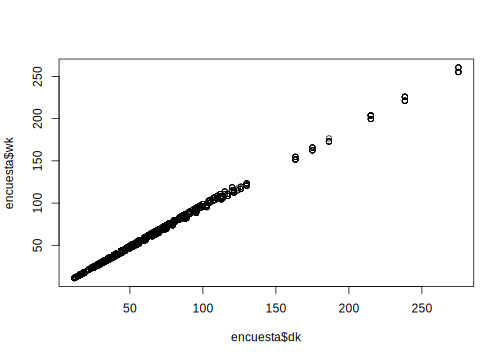
\includegraphics[width=0.7\linewidth]{04-Continuas_files/figure-latex/unnamed-chunk-21-1} \end{center}

\begin{verbatim}
##            lorenz     SE
## L(0)    0.0000000 0.0000
## L(0.05) 0.0068191 0.0008
## L(0.1)  0.0175964 0.0013
## L(0.15) 0.0316596 0.0033
## L(0.2)  0.0492230 0.0041
## L(0.25) 0.0694365 0.0056
## L(0.3)  0.0925871 0.0064
## L(0.35) 0.1181331 0.0071
## L(0.4)  0.1469261 0.0082
## L(0.45) 0.1791978 0.0095
## L(0.5)  0.2158231 0.0106
## L(0.55) 0.2565784 0.0123
## L(0.6)  0.3027002 0.0137
## L(0.65) 0.3537989 0.0149
## L(0.7)  0.4096304 0.0159
## L(0.75) 0.4706565 0.0167
## L(0.8)  0.5398749 0.0177
## L(0.85) 0.6174169 0.0183
## L(0.9)  0.7042464 0.0176
## L(0.95) 0.8151774 0.0152
## L(1)    1.0000000 0.0000
\end{verbatim}

Los argumentos que requiere la función son, inicialmente, los ingresos de los hogares y el diseño muestral complejo. Adicionalmente, se definen una secuencia de probabilidades que define la suma de los cuantiles a calcular (quantiles) y por último, un número que especifica el nivel de confianza para el gráfico (alpha).

\section{Análisis de correlación en encuestas de hogares}\label{anuxe1lisis-de-correlaciuxf3n-en-encuestas-de-hogares}

En el estudio de encuestas de hogares, además de describir variables de forma individual, resulta fundamental analizar cómo se relacionan entre sí. Una de las herramientas más utilizadas es el coeficiente de correlación de Pearson, que mide la fuerza y la dirección de la relación lineal entre dos variables numéricas. Sus valores oscilan entre --1 y 1:

\begin{itemize}
\tightlist
\item
  Un valor positivo indica que ambas variables tienden a aumentar al mismo tiempo.
\item
  Un valor negativo señala que cuando una variable crece, la otra tiende a disminuir.
\item
  Valores próximos a cero sugieren una relación lineal débil o inexistente.
\end{itemize}

Por ejemplo, puede ser de interés analizar si el ingreso de los hogares está asociado con su nivel de gasto, y en qué magnitud.

\subsection{Ajuste al diseño muestral}\label{ajuste-al-diseuxf1o-muestral}

En encuestas complejas, la correlación no puede calcularse como en una muestra simple. Es necesario incorporar los pesos muestrales para que la estimación sea representativa de la población. Este ajuste tiene en cuenta la estratificación, la conglomeración y las probabilidades de selección desiguales.

El cálculo ponderado implica evaluar la covarianza entre las dos variables y dividirla entre el producto de sus desviaciones estándar ponderadas, eliminando así la influencia de las unidades de medida.

\subsection{Expresión formal}\label{expresiuxf3n-formal}

El coeficiente de correlación de Pearson ajustado por pesos se expresa como:

\[\hat{\rho}_{xy} = \frac{\displaystyle \sum_{h=1}^{H} \sum_{i \in s_{1h}} \sum_{k \in s_{hi}} w_{hik} (y_{hik} - \widehat{\bar{Y}})(x_{hik} - \widehat{\bar{X}})} {\sqrt{\displaystyle \sum_{h=1}^{H} \sum_{i \in s_{1h}} \sum_{k \in s_{hi}} w_{hik} (y_{hik} - \widehat{\bar{Y}})^2} \sqrt{\displaystyle \sum_{h=1}^{H} \sum_{i \in s_{1h}} \sum_{k \in s_{hi}} w_{hik} (x_{hik} - \widehat{\bar{X}})^2}}\]

Cuando las variables son categóricas u ordinales, se deben emplear otras medidas de asociación (como el coeficiente de contingencia o de correlación policórica).

\subsection{Implementación en R}\label{implementaciuxf3n-en-r}

El paquete \texttt{survey} cuenta con la función \texttt{svyvar} que permite obtener matrices de covarianzas ponderadas, a partir de las cuales se puede calcular la correlación. Otra opción más directa es usar \texttt{svycor} de paquetes complementarios como \texttt{svycor} o implementar el cálculo manualmente.

Ejemplo con ingreso y gasto de los hogares:

\begin{Shaded}
\begin{Highlighting}[]
\CommentTok{\# Covarianza ponderada}
\NormalTok{svy\_cov }\OtherTok{\textless{}{-}} \FunctionTok{svyvar}\NormalTok{(}\SpecialCharTok{\textasciitilde{}}\NormalTok{Income }\SpecialCharTok{+}\NormalTok{ Expenditure, }\AttributeTok{design =}\NormalTok{ diseno)}
\end{Highlighting}
\end{Shaded}

El resultado entrega la matriz de correlaciones entre las variables analizadas bajo el diseño complejo.

\section{Análisis de la relación entre dos variable continuas}\label{anuxe1lisis-de-la-relaciuxf3n-entre-dos-variable-continuas}

En muchos análisis de variables relacionadas con encuestas de hogares no solo basta con analizar el comportamiento de variables de manera individual, por ejemplo, ingresos medios de hombres y mujeres en un país sino también, analizar la diferencia entre los ingresos de los hombres y las mujeres. Esto último con el fin de ir cerrando la brecha salarial que existe.

En este capítulo se estudiará la prueba de hipótesis para diferencia de medias, se darán las herramientas computacionales para estimar razones y contrastes.

\section{Pruebas para la comparación de grupos}\label{pruebas-para-la-comparaciuxf3n-de-grupos}

El análisis de diferencias entre grupos es un objetivo frecuente en las encuestas de hogares. Un ejemplo clásico es la pregunta: \emph{¿Existen diferencias estadísticamente significativas en el ingreso medio entre hogares dirigidos por hombres y aquellos dirigidos por mujeres?}

Para responder a este tipo de interrogantes se aplican \textbf{pruebas de hipótesis}, procedimientos estadísticos que contrastan afirmaciones sobre parámetros poblacionales a partir de evidencia muestral. En el contexto de encuestas, estas pruebas deben ajustarse al diseño de muestreo (estratificación, conglomerados y ponderación) para garantizar inferencias válidas.

\subsection{Planteamiento general de hipótesis}\label{planteamiento-general-de-hipuxf3tesis}

Una prueba de hipótesis parte de dos proposiciones antagónicas:

\[
\begin{cases}
H_{0}: & \theta = \theta_0 \quad \text{(hipótesis nula)} \\
H_{1}: & \theta \neq \theta_0 \quad \text{(hipótesis alternativa, bilateral)}
\end{cases}
\]

Dependiendo del contexto, \(H_1\) puede plantearse de manera unilateral (\(\theta > \theta_0\) o \(\theta < \theta_0\)). El proceso consiste en evaluar si la evidencia contenida en la muestra es suficiente para rechazar \(H_0\) en favor de \(H_1\).

En muchos casos, los parámetros de interés (medias, proporciones, totales o razones) pueden expresarse como \textbf{combinaciones lineales de estadísticas descriptivas}:

\[
f(\theta_1,\ldots,\theta_J) = \sum_{j=1}^J a_j \theta_j
\]

con estimador:

\[
\hat{f} = \sum_{j=1}^J a_j \hat{\theta}_j
\]

y varianza:

\[
Var(\hat{f}) = \sum_{j=1}^J a_j^2 Var(\hat{\theta}_j) \;+\; 2\sum_{j=1}^{J-1}\sum_{k>j}^J a_j a_k \, Cov(\hat{\theta}_j,\hat{\theta}_k).
\]

Este marco general abarca, entre otros casos, la \textbf{diferencia entre medias poblacionales}.

\subsection{Diferencia de medias poblacionales}\label{diferencia-de-medias-poblacionales}

Sea \(\mu_{(y,d)}\) la media poblacional del dominio \(d\), con \(d=1,2\). El parámetro de interés es:

\[
\Delta = \mu_{(y,1)} - \mu_{(y,2)}.
\]

Por ejemplo, \(\mu_{(y,1)}\) podría ser el ingreso medio en hogares con jefatura masculina y \(\mu_{(y,2)}\) el ingreso medio en hogares con jefatura femenina.

El estimador de la diferencia es:

\[
\hat{\Delta} = \hat{\bar{Y}}_1 - \hat{\bar{Y}}_2,
\]

cuyo error estándar se calcula como:

\[
\hat{se}(\hat{\Delta}) = \sqrt{ \hat{Var}(\hat{\bar{Y}}_1) + \hat{Var}(\hat{\bar{Y}}_2) - 2 \hat{Cov}(\hat{\bar{Y}}_1, \hat{\bar{Y}}_2)}.
\]

\subsection{Estadístico de prueba e intervalo de confianza}\label{estaduxedstico-de-prueba-e-intervalo-de-confianza}

El contraste se realiza con el estadístico:

\[
t = \frac{\hat{\Delta}}{\hat{se}(\hat{\Delta})}, \quad t \sim t_{(df)},
\]

donde los grados de libertad se aproximan como \(df = n - H\) (número de UPMs menos número de estratos).

El intervalo de confianza para \(\Delta\) al nivel \((1-\alpha)\) se define como:

\[
\hat{\Delta} \;\pm\; t_{(1-\alpha/2,df)} \, \hat{se}(\hat{\Delta}).
\]

\subsection{\texorpdfstring{Ejemplo aplicado en \texttt{R}}{Ejemplo aplicado en R}}\label{ejemplo-aplicado-en-r}

En encuestas complejas, estas pruebas se implementan con la función \texttt{svyttest()} del paquete survey, que incorpora automáticamente los ajustes del diseño.

\textbf{Ejemplo 1. Diferencia de ingresos por sexo (población total):}

\begin{Shaded}
\begin{Highlighting}[]
\FunctionTok{svyttest}\NormalTok{(Income }\SpecialCharTok{\textasciitilde{}}\NormalTok{ Sex, }\AttributeTok{design =}\NormalTok{ diseno, }\AttributeTok{level =} \FloatTok{0.95}\NormalTok{)}
\end{Highlighting}
\end{Shaded}

\begin{verbatim}
## 
##  Design-based t-test
## 
## data:  Income ~ Sex
## t = 1.3625, df = 118, p-value = 0.1756
## alternative hypothesis: true difference in mean is not equal to 0
## 95 percent confidence interval:
##  -12.82205  69.38503
## sample estimates:
## difference in mean 
##           28.28149
\end{verbatim}

\textbf{Resultados (ejemplo ficticio):}

\begin{itemize}
\tightlist
\item
  Estadístico t = -1.48
\item
  p-valor = 0.14
\item
  Intervalo de confianza (95\%): (-77.35 , 11.41)
\end{itemize}

Interpretación: con un 95\% de confianza no existe evidencia estadística suficiente para afirmar que los ingresos medios difieren por sexo.

\textbf{Ejemplo 2. Diferencia de ingresos por sexo en zona urbana:}

\begin{Shaded}
\begin{Highlighting}[]
\FunctionTok{svyttest}\NormalTok{(Income }\SpecialCharTok{\textasciitilde{}}\NormalTok{ Sex, }\AttributeTok{design =}\NormalTok{ sub\_Urbano, }\AttributeTok{level =} \FloatTok{0.95}\NormalTok{)}
\end{Highlighting}
\end{Shaded}

\begin{verbatim}
## 
##  Design-based t-test
## 
## data:  Income ~ Sex
## t = 1.5667, df = 63, p-value = 0.1222
## alternative hypothesis: true difference in mean is not equal to 0
## 95 percent confidence interval:
##  -12.31754 101.74023
## sample estimates:
## difference in mean 
##           44.71134
\end{verbatim}

Resultado: nuevamente no se rechaza \(H_0\), lo que indica ausencia de diferencias significativas en el ingreso medio por sexo en la zona urbana.

\textbf{Ejemplo 3. Diferencia de ingresos por sexo, restringido a mayores de 18 años:}

\begin{Shaded}
\begin{Highlighting}[]
\FunctionTok{svyttest}\NormalTok{(Income }\SpecialCharTok{\textasciitilde{}}\NormalTok{ Sex,}
         \AttributeTok{design =}\NormalTok{ diseno }\SpecialCharTok{\%\textgreater{}\%} \FunctionTok{filter}\NormalTok{(Age }\SpecialCharTok{\textgreater{}} \DecValTok{18}\NormalTok{),}
         \AttributeTok{level =} \FloatTok{0.95}\NormalTok{)}
\end{Highlighting}
\end{Shaded}

\begin{verbatim}
## 
##  Design-based t-test
## 
## data:  Income ~ Sex
## t = 1.5263, df = 118, p-value = 0.1296
## alternative hypothesis: true difference in mean is not equal to 0
## 95 percent confidence interval:
##  -10.72746  82.85253
## sample estimates:
## difference in mean 
##           36.06253
\end{verbatim}

Conclusión: tampoco se rechaza \(H_0\). Es decir, no se observa evidencia estadística de diferencias en los ingresos medios entre hombres y mujeres mayores de 18 años.

El procedimiento descrito no se limita a las medias, sino que también puede aplicarse a proporciones, totales, razones o cualquier función diferenciable de totales. En todos los casos, el contraste se fundamenta en la estimación puntual, su varianza (incluyendo covarianzas cuando corresponde) y la comparación con la distribución t ajustada al diseño muestral.

\section{Estimando razones en encuestas de hogares}\label{estimando-razones-en-encuestas-de-hogares}

Un caso particular de una función no lineal de totales es la \textbf{razón poblacional}, definida como el cociente de dos totales poblacionales de características de interés. En encuestas de hogares, este parámetro es relevante cuando, por ejemplo, se requiere conocer la cantidad de hombres por cada mujer, la proporción de ocupados respecto a la población en edad de trabajar, o la cantidad de mascotas por cada hogar. Puesto que la razón es un cociente de totales, tanto el numerador como el denominador son cantidades desconocidas y, por lo tanto, deben estimarse \emph{(Bautista, 1998)}. Formalmente, la razón poblacional se define como:

\[
R = \frac{Y}{X}
\]

y su estimador puntual en el marco de un muestreo complejo se expresa como:

\[
\hat{R} = \frac{\hat{Y}}{\hat{X}}
= \frac{\sum_{h=1}^{H}\sum_{\alpha=1}^{a_{h}}\sum_{i=1}^{n_{h\alpha}}\omega_{h\alpha i} y_{h\alpha i}}
       {\sum_{h=1}^{H}\sum_{\alpha=1}^{a_{h}}\sum_{i=1}^{n_{h\alpha}}\omega_{h\alpha i} x_{h\alpha i}}.
\]

Sin embargo, dado que \(\hat{R}\) es un cociente entre dos estimadores ---es decir, dos variables aleatorias--- el cálculo de su varianza no es trivial. Para ello se emplea la linealización de Taylor, como lo muestra \emph{Gutiérrez (2016)}, o bien métodos de remuestreo. En términos de la función de estimación, se define:

\[
z_{hik} = y_{hik} - \hat{R}x_{hik},
\]

\subsection*{\texorpdfstring{Implementación computacional en \texttt{R}}{Implementación computacional en R}}\label{implementaciuxf3n-computacional-en-r}
\addcontentsline{toc}{subsection}{Implementación computacional en \texttt{R}}

En la práctica, estos cálculos se facilitan gracias a los paquetes especializados. En particular, la función \texttt{survey\_ratio} implementa la estimación de razones y sus varianzas en el marco de encuestas complejas. Para ello es necesario especificar claramente:

\begin{itemize}
\tightlist
\item
  La variable del \textbf{Expenditure} (\texttt{numerator}),
\item
  La variable del \textbf{Income} (\texttt{denominator}),
\item
  El nivel de confianza (\texttt{level}) para los intervalos, y
\item
  Las estadísticas de resumen deseadas (\texttt{vartype}).
\end{itemize}

A continuación, se ilustra cómo estimar la razón entre el gasto y el ingreso de los hogares:

\begin{Shaded}
\begin{Highlighting}[]
\NormalTok{diseno }\SpecialCharTok{\%\textgreater{}\%} \FunctionTok{summarise}\NormalTok{(}
    \AttributeTok{Razon =}  \FunctionTok{survey\_ratio}\NormalTok{(}
      \AttributeTok{numerator =}\NormalTok{ Expenditure,}
      \AttributeTok{denominator =}\NormalTok{ Income,}
      \AttributeTok{level =} \FloatTok{0.95}\NormalTok{,}
    \AttributeTok{vartype =}  \FunctionTok{c}\NormalTok{(}\StringTok{"se"}\NormalTok{, }\StringTok{"ci"}\NormalTok{)}
\NormalTok{    ))}
\end{Highlighting}
\end{Shaded}

\begin{verbatim}
## # A tibble: 1 x 4
##   Razon Razon_se Razon_low Razon_upp
##   <dbl>    <dbl>     <dbl>     <dbl>
## 1 0.649   0.0232     0.603     0.695
\end{verbatim}

\subsection*{Interpretación aplicada}\label{interpretaciuxf3n-aplicada}
\addcontentsline{toc}{subsection}{Interpretación aplicada}

Las razones permiten expresar la relación entre dos variables, lo cual resulta especialmente útil para construir indicadores comparativos y de seguimiento. Un ejemplo directo en encuestas de hogares es la razón \textbf{gasto/ingreso}, que ayuda a identificar patrones de consumo y niveles de sostenibilidad económica de los hogares.

Más allá de este caso, las razones también se utilizan en marcos internacionales. Por ejemplo, el \textbf{Indicador 2.1.1 de los Objetivos de Desarrollo Sostenible (ODS)} ---prevalencia de subalimentación--- se calcula a partir de la razón entre el consumo de alimentos, medido en calorías ingeridas, y los requerimientos energéticos mínimos de la dieta, determinados según edad, sexo y nivel de actividad física.

De esta forma, las razones constituyen una herramienta central para transformar los resultados de encuestas en indicadores significativos que facilitan el análisis de realidades socioeconómicas y poblacionales.

Como se puede observar, la razón entre el gasto y el ingreso es, aproximando, 0.71. Lo que implica que por cada unidad 100 unidades monetarias que le ingrese al hogar, se gastan 71 unidades, consiguiendo un intervalo de confianza al 95\% de 0.65 y 0.76.

Si ahora el objetivo es estimar la razón entre mujeres y hombres en la base de ejemplo, se realiza de la siguiente manera:

\begin{Shaded}
\begin{Highlighting}[]
\NormalTok{diseno }\SpecialCharTok{\%\textgreater{}\%} \FunctionTok{summarise}\NormalTok{(}
    \AttributeTok{Razon =}  \FunctionTok{survey\_ratio}\NormalTok{(}
      \AttributeTok{numerator =}\NormalTok{ (Sex }\SpecialCharTok{==} \StringTok{"Female"}\NormalTok{),}
      \AttributeTok{denominator =}\NormalTok{ (Sex }\SpecialCharTok{==} \StringTok{"Male"}\NormalTok{),}
      \AttributeTok{level =} \FloatTok{0.95}\NormalTok{,}
    \AttributeTok{vartype =}  \FunctionTok{c}\NormalTok{(}\StringTok{"se"}\NormalTok{, }\StringTok{"ci"}\NormalTok{)}
\NormalTok{    ))}
\end{Highlighting}
\end{Shaded}

\begin{verbatim}
## # A tibble: 1 x 4
##   Razon Razon_se Razon_low Razon_upp
##   <dbl>    <dbl>     <dbl>     <dbl>
## 1  1.11   0.0351      1.04      1.18
\end{verbatim}

Como la variable sexo en la base de datos es una variable categórica, se tuvo la necesidad de generar las variables dummys para su cálculo realizando, Sex == ``Female'' para el caso de las mujeres y Sex == ``Male'' para el caso de los hombres. Los resultados del ejercicio anterior muestran que en la base de datos hay más mujeres que hombres, generando una razón de 1.13. Esto significa que, por cada 100 hombres hay aproximadamente 113 mujeres con un intervalo que varía entre 1.04 y 1.21.

Si se desea hacer la razón de mujeres y hombres pero en la zona rural, se haría de la siguiente manera:

\begin{Shaded}
\begin{Highlighting}[]
\NormalTok{sub\_Rural }\SpecialCharTok{\%\textgreater{}\%} \FunctionTok{summarise}\NormalTok{(}
    \AttributeTok{Razon =}  \FunctionTok{survey\_ratio}\NormalTok{(}
      \AttributeTok{numerator =}\NormalTok{ (Sex }\SpecialCharTok{==} \StringTok{"Female"}\NormalTok{),}
      \AttributeTok{denominator =}\NormalTok{ (Sex }\SpecialCharTok{==} \StringTok{"Male"}\NormalTok{),}
      \AttributeTok{level =} \FloatTok{0.95}\NormalTok{,}
    \AttributeTok{vartype =}  \FunctionTok{c}\NormalTok{(}\StringTok{"se"}\NormalTok{, }\StringTok{"ci"}\NormalTok{)}
\NormalTok{    ))}
\end{Highlighting}
\end{Shaded}

\begin{verbatim}
## # A tibble: 1 x 4
##   Razon Razon_se Razon_low Razon_upp
##   <dbl>    <dbl>     <dbl>     <dbl>
## 1  1.07   0.0352     0.997      1.14
\end{verbatim}

Obteniendo nuevamente que hay más mujeres que hombres. Ahora bien, otro análisis de interés es estimar la razón de gastos pero solo en la población femenina. A continuación, se presentan los códigos computacionales.

\begin{Shaded}
\begin{Highlighting}[]
\NormalTok{sub\_Mujer }\SpecialCharTok{\%\textgreater{}\%} \FunctionTok{summarise}\NormalTok{(}
    \AttributeTok{Razon =}  \FunctionTok{survey\_ratio}\NormalTok{(}
      \AttributeTok{numerator =}\NormalTok{ Expenditure,}
      \AttributeTok{denominator =}\NormalTok{ Income,}
      \AttributeTok{level =} \FloatTok{0.95}\NormalTok{,}
    \AttributeTok{vartype =}  \FunctionTok{c}\NormalTok{(}\StringTok{"se"}\NormalTok{, }\StringTok{"ci"}\NormalTok{)}
\NormalTok{    ))}
\end{Highlighting}
\end{Shaded}

\begin{verbatim}
## # A tibble: 1 x 4
##   Razon Razon_se Razon_low Razon_upp
##   <dbl>    <dbl>     <dbl>     <dbl>
## 1 0.658   0.0199     0.619     0.698
\end{verbatim}

Dando como resultado que por cada 100 unidades monetarias que le ingresan a las mujeres se gastan 70 con un intervalo de confianza entre 0.65 y 0.76. Por último, análogamente para los hombres, la razón de gastos resulta muy similar que para las mujeres.

\begin{Shaded}
\begin{Highlighting}[]
\NormalTok{sub\_Hombre }\SpecialCharTok{\%\textgreater{}\%} \FunctionTok{summarise}\NormalTok{(}
    \AttributeTok{Razon =}  \FunctionTok{survey\_ratio}\NormalTok{(}
      \AttributeTok{numerator =}\NormalTok{ Expenditure,}
      \AttributeTok{denominator =}\NormalTok{ Income,}
      \AttributeTok{level =} \FloatTok{0.95}\NormalTok{,}
    \AttributeTok{vartype =}  \FunctionTok{c}\NormalTok{(}\StringTok{"se"}\NormalTok{, }\StringTok{"ci"}\NormalTok{)}
\NormalTok{    ))}
\end{Highlighting}
\end{Shaded}

\begin{verbatim}
## # A tibble: 1 x 4
##   Razon Razon_se Razon_low Razon_upp
##   <dbl>    <dbl>     <dbl>     <dbl>
## 1 0.639   0.0288     0.582     0.696
\end{verbatim}

\section{Estimando contrastes en encuestas de hogares}\label{estimando-contrastes-en-encuestas-de-hogares}

En muchas ocasiones, en encuestas de hogares se requiere comparar más de dos poblaciones al mismo tiempo, por ejemplo, comparar los ingresos medios de los hogares en 3 regiones o municipalidades en la postpandemia con el fin de verificar y sectorizar aquellas municipalidades o regiones donde más impacto en el desempleo y falta de ingresos tuvo el Covid-19 en los hogares. En casos como estos la diferencia de media que estudiamos en capítulos anteriores se queda corta dado que permite solo comprar parejas de poblaciones y por ende que, hacer contraste resulta una muy buena alternativa para abordar este tipo de problemas.

Recurriendo en las definiciones que se han trabajado en este capítulo, un contraste es una combinación lineal de parámetros de la forma:

\begin{eqnarray*}
f\left(\theta _{1},\theta_{2},...,\theta_{j}\right) & = & \sum_{j=1}^{J}a_{j}\theta_{j}
\end{eqnarray*}

Una estimación de esta función está dada por:

\begin{eqnarray*}
f\left(\hat{\theta}_{1},\hat{\theta}_{2},...,\hat{\theta}_{j}\right) & = & \sum_{j=1}^{J}a_{j}\hat{\theta}_{j}
\end{eqnarray*}

cuya varianza del estimador se calcula como sigue:

\begin{eqnarray*}
var\left(\sum_{j=1}^{J}a_{j}\hat{\theta}_{j}\right) & = & \sum_{j=1}^{J}a_{j}^{2}var\left(\hat{\theta}_{j}\right)+2\times\sum_{j=1}^{J-1}\sum_{k>j}^{J}a_{j}a_{k}\,cov\left(\hat{\theta}_{j},\hat{\theta}_{k}\right)
\end{eqnarray*}

Los procedimientos metodológicos para implementar los contrastes en diseños de muestreo complejos están desarrolladas en la función \texttt{svycontrast}. A continuación, se muestra el uso de dicha función para el cálculo de contraste en la base de datos de ejemplo, comparando el promedio de ingresos por región.

Como primer ejemplo, se realizará la comparación de dos poblaciones, las regiones Norte y Sur (\(\bar{Y}_{Norte} - \bar{Y}_{Sur}\)) y luego sí se compararán todas las regiones.

Puesto que esto es un contraste en donde hay 5 regiones y solo se construirá el contraste para la región Norte y la Sur, el contraste queda definido de la siguiente manera:

\begin{eqnarray*}
 & 1\times\hat{\bar{Y}}_{Norte}+\left(-1\right)\times\hat{\bar{Y}}_{Sur}+0\times\hat{\bar{Y}}_{Centro}+0\times\hat{\bar{Y}}_{Occidente}+0\times\hat{\bar{Y}}_{Oriente}
\end{eqnarray*}

que de forma matricial queda de la siguiente manera:

\begin{eqnarray*}
 & \left[1,\,-1,\,0,\,0,\,0\right]\times\left[\begin{array}{c}
\hat{\bar{Y}}_{Norte}\\
\hat{\bar{Y}}_{Sur}\\
\hat{\bar{Y}}_{Centro}\\
\hat{\bar{Y}}_{Occidente}\\
\hat{\bar{Y}}_{Oriente}
\end{array}\right]
\end{eqnarray*}

Como se puede observar, en este caso el vector de contraste es \(\left[1,\,-1,\,0,\,0,\,0\right]\).

Ahora bien, para realizar el procesos de la construcción del estimador del contraste y su varianza estimada paso a paso se inicia con calcular las medias estimadas por región con la función \texttt{svyby} como se muestra a continuación:

\begin{Shaded}
\begin{Highlighting}[]
\NormalTok{prom\_region }\OtherTok{\textless{}{-}} \FunctionTok{svyby}\NormalTok{(}\AttributeTok{formula =} \SpecialCharTok{\textasciitilde{}}\NormalTok{Income,}
                      \AttributeTok{by =} \SpecialCharTok{\textasciitilde{}}\NormalTok{Region,}
                      \AttributeTok{design =}\NormalTok{ diseno,}
                      \AttributeTok{FUN =}\NormalTok{ svymean,}
                      \AttributeTok{na.rm=}\NormalTok{T,}
                      \AttributeTok{covmat =} \ConstantTok{TRUE}\NormalTok{,}
                      \AttributeTok{vartype =} \FunctionTok{c}\NormalTok{(}\StringTok{"se"}\NormalTok{, }\StringTok{"ci"}\NormalTok{))}
\NormalTok{prom\_region}
\end{Highlighting}
\end{Shaded}

\begin{verbatim}
##              Region   Income       se     ci_l     ci_u
## Norte         Norte 552.3637 55.35987 443.8603 660.8670
## Sur             Sur 625.7740 62.40574 503.4610 748.0870
## Centro       Centro 650.7820 61.46886 530.3053 771.2588
## Occidente Occidente 517.0071 46.22077 426.4161 607.5982
## Oriente     Oriente 541.7543 71.66487 401.2938 682.2149
\end{verbatim}

La función \texttt{svyby} permite aplicar una función, en este caso la media (svymean) por región (by) utilizando el diseño muestral empleado (design). Las demás componentes de la función ya se han utilizado previamente. Como resultado de aplicar esta función se obtienen las medias estimadas de los ingresos por región. Se tomarán solo los ingresos medios estimados de las regiones Norte y Sur y calcularemos su diferencia:

\begin{Shaded}
\begin{Highlighting}[]
\CommentTok{\# Paso 1: diferencia de estimaciones (Norte {-} Sur)}
\FloatTok{552.4} \SpecialCharTok{{-}} \FloatTok{625.8}
\end{Highlighting}
\end{Shaded}

\begin{verbatim}
## [1] -73.4
\end{verbatim}

El paso siguiente es calcular la matriz de varianzas y covarianzas y de allí extraer las varianzas y covarianzas de las regiones Norte y Sur:

\begin{Shaded}
\begin{Highlighting}[]
\CommentTok{\# Paso 2: Matriz de varianzas y covarianzas}
\FunctionTok{vcov}\NormalTok{(prom\_region)}
\end{Highlighting}
\end{Shaded}

\begin{verbatim}
##              Norte      Sur  Centro Occidente  Oriente
## Norte     3064.715    0.000    0.00     0.000    0.000
## Sur          0.000 3894.476    0.00     0.000    0.000
## Centro       0.000    0.000 3778.42     0.000    0.000
## Occidente    0.000    0.000    0.00  2136.359    0.000
## Oriente      0.000    0.000    0.00     0.000 5135.854
\end{verbatim}

Para calcular el error estándar de la diferencia (contraste) se usará las propiedades de la varianza como es
\(se\left(\hat{\bar{y}}_{Norte}-\hat{\bar{y}}_{Sur}\right)=\sqrt{var\left(\hat{\bar{y}}_{Norte}\right)+var\left(\hat{\bar{y}}_{Sur}\right)-2\,cov\left(\hat{\bar{y}}_{Norte},\hat{\bar{y}}_{Sur}\right)}\) tenemos:

\begin{Shaded}
\begin{Highlighting}[]
\FunctionTok{sqrt}\NormalTok{(}\DecValTok{3065} \SpecialCharTok{+} \DecValTok{3894} \SpecialCharTok{{-}} \DecValTok{2}\SpecialCharTok{*}\DecValTok{0}\NormalTok{)}
\end{Highlighting}
\end{Shaded}

\begin{verbatim}
## [1] 83.42062
\end{verbatim}

Finalmente, la función \texttt{svycontrast} nos devuelve el contraste estimado y su error estándar. Los argumentos de esta función son los promedios de los ingresos estimados (stat) y las constantes de contraste (contrasts).

\begin{Shaded}
\begin{Highlighting}[]
\FunctionTok{svycontrast}\NormalTok{(}\AttributeTok{stat =}\NormalTok{ prom\_region,}
            \AttributeTok{contrasts =} \FunctionTok{list}\NormalTok{(}\AttributeTok{diff\_NS =} \FunctionTok{c}\NormalTok{(}\DecValTok{1}\NormalTok{, }\SpecialCharTok{{-}}\DecValTok{1}\NormalTok{, }\DecValTok{0}\NormalTok{, }\DecValTok{0}\NormalTok{, }\DecValTok{0}\NormalTok{))) }\SpecialCharTok{\%\textgreater{}\%}
            \FunctionTok{data.frame}\NormalTok{()}
\end{Highlighting}
\end{Shaded}

\begin{verbatim}
##          contrast  diff_NS
## diff_NS -73.41034 83.42176
\end{verbatim}

Obteniendo como resultado que los ingresos medios estimados para la región Sur es 73.4 unidades monetarias mayor que los ingresos en la región Norte con un error estándar de 83.42 unidades.

Ahora bien, si el objetivo es estimar los siguientes contrastes:

\begin{itemize}
\tightlist
\item
  \(\bar{Y}_{Norte} - \bar{Y}_{Centro}\),
\item
  \(\bar{Y}_{Sur}-\bar{Y}_{Centro}\)
\item
  \(\bar{Y}_{Occidente}-\bar{Y}_{Oriente}\)
\end{itemize}

Que escritas de forma matricial se tiene:

\[
\left[\begin{array}{ccccc}
1 & 0 & -1 & 0 & 0\\
0 & 1 & -1 & 0 & 0\\
0 & 0 & 0 & 1 & -1
\end{array}\right]
\]

Ahora, aplicando la función \texttt{svycontrast} en R se obtiene:

\begin{Shaded}
\begin{Highlighting}[]
\FunctionTok{svycontrast}\NormalTok{(}\AttributeTok{stat =}\NormalTok{ prom\_region,}
            \AttributeTok{contrasts =} \FunctionTok{list}\NormalTok{(}
                             \AttributeTok{Norte\_sur =} \FunctionTok{c}\NormalTok{(}\DecValTok{1}\NormalTok{, }\DecValTok{0}\NormalTok{, }\SpecialCharTok{{-}}\DecValTok{1}\NormalTok{, }\DecValTok{0}\NormalTok{, }\DecValTok{0}\NormalTok{),}
                             \AttributeTok{Sur\_centro =} \FunctionTok{c}\NormalTok{(}\DecValTok{0}\NormalTok{, }\DecValTok{1}\NormalTok{, }\SpecialCharTok{{-}}\DecValTok{1}\NormalTok{, }\DecValTok{0}\NormalTok{, }\DecValTok{0}\NormalTok{),}
                             \AttributeTok{Occidente\_Oriente =} \FunctionTok{c}\NormalTok{(}\DecValTok{0}\NormalTok{, }\DecValTok{0}\NormalTok{, }\DecValTok{0}\NormalTok{, }\DecValTok{1}\NormalTok{, }\SpecialCharTok{{-}}\DecValTok{1}\NormalTok{))) }\SpecialCharTok{\%\textgreater{}\%}                               \FunctionTok{data.frame}\NormalTok{()}
\end{Highlighting}
\end{Shaded}

\begin{verbatim}
##                    contrast       SE
## Norte_sur         -98.41834 82.72324
## Sur_centro        -25.00800 87.59507
## Occidente_Oriente -24.74720 85.27727
\end{verbatim}

De lo cual se puede concluir que, las regiones con los ingresos medios de los hogares más similares son la región sur y la región centro.

También es posible construir contraste en variables que estén correlacionadas. Por ejemplo, Ingreso y Sexo. Como se hizo en el ejemplo anterior, se inicia con el promedio estimado por sexo.

\begin{Shaded}
\begin{Highlighting}[]
\NormalTok{prom\_sexo }\OtherTok{\textless{}{-}} \FunctionTok{svyby}\NormalTok{(}\AttributeTok{formula =} \SpecialCharTok{\textasciitilde{}}\NormalTok{Income,}
                   \AttributeTok{by =} \SpecialCharTok{\textasciitilde{}}\NormalTok{Sex,}
                   \AttributeTok{design =}\NormalTok{ diseno,}
                   \AttributeTok{FUN =}\NormalTok{ svymean,}
                   \AttributeTok{na.rm=}\NormalTok{T,}
                   \AttributeTok{covmat =} \ConstantTok{TRUE}\NormalTok{,}
                   \AttributeTok{vartype =} \FunctionTok{c}\NormalTok{(}\StringTok{"se"}\NormalTok{, }\StringTok{"ci"}\NormalTok{))}
\NormalTok{prom\_sexo}
\end{Highlighting}
\end{Shaded}

\begin{verbatim}
##           Sex   Income       se     ci_l     ci_u
## Female Female 557.5681 25.82995 506.9423 608.1939
## Male     Male 585.8496 34.58759 518.0592 653.6400
\end{verbatim}

El contraste a estimar es:

\[ \bar{Y}_{F} - \bar{Y}_{M}\]
Por tanto, usando la función \texttt{svycontrast} se obtiene el contraste estimado:

\begin{Shaded}
\begin{Highlighting}[]
\FunctionTok{svycontrast}\NormalTok{(}\AttributeTok{stat =}\NormalTok{ prom\_sexo,}
            \AttributeTok{contrasts =} \FunctionTok{list}\NormalTok{(}\AttributeTok{diff\_Sexo =} \FunctionTok{c}\NormalTok{(}\DecValTok{1}\NormalTok{, }\SpecialCharTok{{-}}\DecValTok{1}\NormalTok{))) }\SpecialCharTok{\%\textgreater{}\%}
            \FunctionTok{data.frame}\NormalTok{()}
\end{Highlighting}
\end{Shaded}

\begin{verbatim}
##            contrast diff_Sexo
## diff_Sexo -28.28149  20.75651
\end{verbatim}

Obteniendo como resultado que, en promedio, los hombres obtienen 28.3 unidades monetarias más que las mujeres con una desviación de 20.76.

Otra posibilidad es poder obtener resultados agregados, por ejemplo:

\(\hat{\bar{y}}_{Norte}+\hat{\bar{y}}_{Sur} +\hat{\bar{y}}_{Centro}\)

\begin{Shaded}
\begin{Highlighting}[]
\NormalTok{sum\_region }\OtherTok{\textless{}{-}} \FunctionTok{svyby}\NormalTok{( }\SpecialCharTok{\textasciitilde{}}\NormalTok{ Income,  }\SpecialCharTok{\textasciitilde{}}\NormalTok{ Region,}
\NormalTok{                     diseno, svytotal, }\AttributeTok{na.rm =}\NormalTok{ T,}
                     \AttributeTok{covmat =} \ConstantTok{TRUE}\NormalTok{,}
                     \AttributeTok{vartype =} \FunctionTok{c}\NormalTok{(}\StringTok{"se"}\NormalTok{, }\StringTok{"ci"}\NormalTok{))}
\NormalTok{sum\_region}
\end{Highlighting}
\end{Shaded}

\begin{verbatim}
##              Region   Income      se     ci_l     ci_u
## Norte         Norte 14277323 1507575 11322530 17232115
## Sur             Sur 16068151 1877989 12387359 19748942
## Centro       Centro 16483319 2383556 11811634 21155003
## Occidente Occidente 16853540 1823807 13278944 20428135
## Oriente     Oriente 22111335 2833460 16557856 27664814
\end{verbatim}

La matriz de contraste queda como:
\[
\left[\begin{array}{cccccc}
1 & 1 & 1 & 0 & 0
\end{array}\right]
\]
el procedimiento en R es:

\begin{Shaded}
\begin{Highlighting}[]
\FunctionTok{svycontrast}\NormalTok{(}\AttributeTok{stat =}\NormalTok{ sum\_region,}
            \AttributeTok{contrasts =} \FunctionTok{list}\NormalTok{(}
                             \AttributeTok{Agregado\_NCS =} \FunctionTok{c}\NormalTok{(}\DecValTok{1}\NormalTok{, }\DecValTok{1}\NormalTok{, }\DecValTok{1}\NormalTok{, }\DecValTok{0}\NormalTok{, }\DecValTok{0}\NormalTok{))) }\SpecialCharTok{\%\textgreater{}\%}                        \FunctionTok{data.frame}\NormalTok{()}
\end{Highlighting}
\end{Shaded}

\begin{verbatim}
##              contrast Agregado_NCS
## Agregado_NCS 46828792      3388357
\end{verbatim}

Por otro lado, si se desean obtener los promedios por categorías. Por ejemplo:

\[
\hat{\bar{y}}_{Edad} = \frac{1}{k}\sum_{k=1}^K\hat{\bar{y}}_{k}
\]
donde \(K\) es el número de categorías de la variable. En R se hace de la siguiente manera:

\begin{Shaded}
\begin{Highlighting}[]
\NormalTok{prom\_edad }\OtherTok{\textless{}{-}} \FunctionTok{svyby}\NormalTok{(}\AttributeTok{formula =} \SpecialCharTok{\textasciitilde{}}\NormalTok{Income,}
                   \AttributeTok{by =} \SpecialCharTok{\textasciitilde{}}\NormalTok{CatAge,}
                   \AttributeTok{design =}\NormalTok{  diseno,}
                   \AttributeTok{FUN =}\NormalTok{ svymean,}
                   \AttributeTok{na.rm=}\NormalTok{T,}
                   \AttributeTok{covmat =} \ConstantTok{TRUE}\NormalTok{)}
\NormalTok{prom\_edad}
\end{Highlighting}
\end{Shaded}

\begin{verbatim}
##              CatAge   Income       se
## 0-5             0-5 463.7715 28.86795
## 6-15           6-15 511.6179 34.88031
## 16-30         16-30 607.2917 37.41561
## 31-45         31-45 573.4167 26.94744
## 46-60         46-60 763.0610 58.97170
## Más de 60 Más de 60 466.6133 31.20795
\end{verbatim}

Cuya matriz de contraste estaría dada por:
\[
\left[\begin{array}{cccccc}
\frac{1}{6} & \frac{1}{6} & \frac{1}{6} & \frac{1}{6} & \frac{1}{6} & \frac{1}{6}
\end{array}\right]
\]

El procedimiento en R es:

\begin{Shaded}
\begin{Highlighting}[]
\FunctionTok{svycontrast}\NormalTok{(}\AttributeTok{stat =}\NormalTok{ prom\_edad,}
            \AttributeTok{contrasts =} \FunctionTok{list}\NormalTok{(}
                             \AttributeTok{agregado\_edad =} \FunctionTok{c}\NormalTok{(}\DecValTok{1}\SpecialCharTok{/}\DecValTok{6}\NormalTok{, }\DecValTok{1}\SpecialCharTok{/}\DecValTok{6}\NormalTok{, }\DecValTok{1}\SpecialCharTok{/}\DecValTok{6}\NormalTok{, }\DecValTok{1}\SpecialCharTok{/}\DecValTok{6}\NormalTok{, }\DecValTok{1}\SpecialCharTok{/}\DecValTok{6}\NormalTok{, }\DecValTok{1}\SpecialCharTok{/}\DecValTok{6}\NormalTok{)))             }\SpecialCharTok{\%\textgreater{}\%} \FunctionTok{data.frame}\NormalTok{()}
\end{Highlighting}
\end{Shaded}

\begin{verbatim}
##               contrast agregado_edad
## agregado_edad 564.2954      25.40408
\end{verbatim}

Puesto que los contrastes, como ya se mencionó, es una función lineal de parámetros, se puede también realizar contraste con parámetros tipo razón. Por ejemplo, la relación de gastos contra ingresos por sexo. A continuación, se muestran los códigos computacionales:

\begin{Shaded}
\begin{Highlighting}[]
\NormalTok{razon\_sexo }\OtherTok{\textless{}{-}} \FunctionTok{svyby}\NormalTok{( }\AttributeTok{formula =} \SpecialCharTok{\textasciitilde{}}\NormalTok{Income,}
                     \AttributeTok{by =} \SpecialCharTok{\textasciitilde{}}\NormalTok{Sex,}
                     \AttributeTok{denominator =} \SpecialCharTok{\textasciitilde{}}\NormalTok{Expenditure,}
                     \AttributeTok{design =}\NormalTok{ diseno,}
                     \AttributeTok{FUN =}\NormalTok{ svyratio,}
                     \AttributeTok{na.rm=}\NormalTok{T, }\AttributeTok{covmat =} \ConstantTok{TRUE}\NormalTok{,}
                     \AttributeTok{vartype =} \FunctionTok{c}\NormalTok{(}\StringTok{"se"}\NormalTok{, }\StringTok{"ci"}\NormalTok{))}
\NormalTok{razon\_sexo}
\end{Highlighting}
\end{Shaded}

\begin{verbatim}
##           Sex Income/Expenditure se.Income/Expenditure     ci_l     ci_u
## Female Female           1.519060            0.04582607 1.429243 1.608878
## Male     Male           1.564762            0.07044239 1.426698 1.702827
\end{verbatim}

Cuya estimación de contraste sería:

\begin{Shaded}
\begin{Highlighting}[]
\FunctionTok{svycontrast}\NormalTok{(}\AttributeTok{stat =}\NormalTok{ razon\_sexo,}
            \AttributeTok{contrasts =} \FunctionTok{list}\NormalTok{(}
                             \AttributeTok{diff\_sexo =} \FunctionTok{c}\NormalTok{(}\DecValTok{1}\NormalTok{, }\SpecialCharTok{{-}}\DecValTok{1}\NormalTok{))) }\SpecialCharTok{\%\textgreater{}\%} \FunctionTok{data.frame}\NormalTok{()}
\end{Highlighting}
\end{Shaded}

\begin{verbatim}
##              contrast  diff_sexo
## diff_sexo -0.04570214 0.04163431
\end{verbatim}

de lo que se puede concluir que la diferencia de las proporciones es 0.045 en favor de los hombres.

\chapter{Referencias}\label{referencias}

\begin{itemize}
\item
  Asparouhov, T., \& Muthen, B. (2006, August). Multilevel modeling of complex survey data. In Proceedings of the joint statistical meeting in Seattle (pp.~2718-2726).
\item
  Asparouhov, T. (2006). General multi-level modeling with sampling weights. Communications in Statistics---Theory and Methods, 35(3), 439-460.
\item
  Pfeffermann, D., Skinner, C. J., Holmes, D. J., Goldstein, H., \& Rasbash, J. (1998). Weighting for unequal selection probabilities in multilevel models. Journal of the Royal Statistical Society: series B (statistical methodology), 60(1), 23-40.
\item
  Cai, T. (2013). Investigation of ways to handle sampling weights for multilevel model analyses. Sociological Methodology, 43(1), 178-219.
\item
  Finch, W. H., Bolin, J. E., \& Kelley, K. (2019). Multilevel modeling using R. Crc Press.
\item
  Merlo, J., Chaix, B., Ohlsson, H., Beckman, A., Johnell, K., Hjerpe, P., \ldots{} \& Larsen, K. (2006). A brief conceptual tutorial of multilevel analysis in social epidemiology: using measures of clustering in multilevel logistic regression to investigate contextual phenomena. Journal of Epidemiology \& Community Health, 60(4), 290-297.
\item
  Sarndal, C., Swensson, B. \&Wretman, J. (1992), Model Assisted Survey Sampling, Springer, New York.
\item
  Rojas, H. A. G. (2016). Estrategias de muestreo: diseño de encuestas y estimación de parámetros. Ediciones de la U.
\item
  Santana Sepúlveda, S., \& Mateos Farfán, E. (2014). El arte de programar en R: un lenguaje para la estadística.
\item
  Lumley, T. (2011). Complex surveys: a guide to analysis using R. John Wiley \& Sons.
\item
  Bache, S. M., Wickham, H., Henry, L., \& Henry, M. L. (2022). Package `magrittr'.
\item
  Tellez Piñerez, C. F., \& Lemus Polanía, D. F. (2015). Estadística Descriptiva y Probabilidad con aplicaciones en R. Fundación Universitaria Los Libertadore.
\item
  Groves, R. M., Fowler Jr, F. J., Couper, M. P., Lepkowski, J. M., Singer, E., \& Tourangeau, R. (2011). Survey methodology. John Wiley \& Sons.
\item
  Tille, Y. \& Ardilly, P. (2006), Sampling Methods: Exercises and Solutions, Springer.
\item
  Gambino, J. G., \& do Nascimento Silva, P. L. (2009). Sampling and estimation in household surveys. In Handbook of Statistics (Vol. 29, pp.~407-439). Elsevier.
\item
  Cochran, W. G. (1977) \emph{Sampling Techniques}. John Wiley and Sons.
\item
  Gutiérrez, H. A. (2017) \texttt{TeachingSampling}. \emph{R package}.
\item
  Wickham, H., Chang, W., \& Wickham, M. H. (2016). Package `ggplot2'. Create elegant data visualisations using the grammar of graphics. Version, 2(1), 1-189.
\item
  Lumley, T. (2020). Package `survey'. Available at the following link: \url{https://cran}. r-project. org.
\item
  Hansen, M. H., \& Steinberg, J. (1956). Control of errors in surveys. Biometrics, 12(4), 462-474.
\item
  Heeringa, S. G., West, B. T., \& Berglund, P. A. (2017). Applied survey data analysis. chapman and hall/CRC.
\item
  Valliant, R., Dever, J.A., and Kreuter, F., Practical Tools for Designing and Weighting Survey Samples, Springer, New York, 2013.
\item
  Valliant, R., Dorfman, A.H., and Royall, R.M., Finite Population Sampling and Inference: A Prediction Approach, John Wiley \& Sons, New York, 2000.
\item
  Loomis, D., Richardson, D.B., and Elliott, L., Poisson regression analysis of ungrouped data, Occupational and Environmental Medicine, 62, 325--329, 2005.
\item
  Kovar, J.G., Rao, J.N.K., and Wu, C.F.J., Bootstrap and other methods to measure errors in survey estimates, Canadian Journal of Statistics, 16(Suppl.), 25--45, 1988.
\item
  Binder, D.A. and Kovacevic, M.S., Estimating some measures of income inequality from survey data: An application of the estimating equations approach, Survey Methodology, 21(2), 137--145, 1995.
\item
  Kovacevic, M. S., \& Binder, D. A. (1997). Variance estimation for measures of income inequality and polarization-the estimating equations approach. Journal of Official Statistics, 13(1), 41.
\item
  Bautista, J. (1998), Diseños de muestreo estadístico, Universidad Nacional de Colombia.
\item
  Monroy, L. G. D., Rivera, M. A. M., \& Dávila, L. R. L. (2018). Análisis estadístico de datos categóricos. Universidad Nacional de Colombia.
\item
  Kish, L. and Frankel, M.R., Inference from complex samples, Journal of the Royal Statistical Society, Series B, 36, 1--37, 1974.
\item
  Fuller, W.A., Regression analysis for sample survey, Sankyha, Series C, 37, 117--132, 1975.
\item
  Shah, B.V., Holt, M.M., and Folsom, R.F., Inference about regression models from sample survey data, Bulletin of the International Statistical Institute, 41(3), 43--57, 1977.
\item
  Skinner, C.J., Holt, D., and Smith, T.M.F., Analysis of Complex Surveys, John Wiley \& Sons, New York, 1989.
\item
  Binder, D.A., On the variances of asymptotically normal estimators from complex surveys, International Statistical Review, 51, 279--292, 1983.
\item
  Fuller, W.A., Regression estimation for survey samples (with discussion), Survey Methodology, 28(1), 5--23, 2002.
\item
  Pfeffermann, D., Modelling of complex survey data: Why model? Why is it a problem? How can we approach it? Survey Methodology, 37(2), 115--136, 2011.
\item
  Wolter, K.M., Introduction to Variance Estimation (2nd ed.), Springer-Verlag, New York, 2007.
\item
  Tellez, C. F., \& Morales, M. A. (2016). Modelos Estadísticos lineales con aplicaciones en R. Ediciones de la U.
\item
  Fay, R.E., On adjusting the Pearson Chi-square statistic for cluster sampling, In Proceedings of the Social Statistics Section, American Statistical Association, Washington, DC, 402--405, 1979.
\item
  Fay, R.E., A jack-knifed chi-squared test for complex samples, Journal of the American Statistical Association, 80, 148--157, 1985.
\item
  Fellegi, I.P., Approximate tests of independence and goodness of fit based on stratified multistage samples, Journal of the American Statistical Association, 75, 261--268, 1980.
\item
  Thomas, D.R. and Rao, J.N.K., Small-sample comparisons of level and power for simple goodness-of-fit statistics under cluster sampling, Journal of the American Statistical Association, 82, 630--636, 1987.
\item
  Rao, J.N.K. and Scott, A.J., On chi-squared test for multiway contingency tables with cell proportions estimated from survey data, The Annals of Statistics, 12, 46--60, 1984.
\item
  Van Buuren, S., Flexible Imputation of Missing Data, Chapman \& Hall, Boca Raton, FL, 2012.
\item
  Carpenter, J.R. and Kenward, M.G., Multiple Imputation and Its Application, John Wiley \& Sons, Chichester, West Sussex, UK, 2013.
\item
  Berglund, P.A. and Heeringa, S.G., Multiple Imputation of Missing Data Using SAS®, SAS Institute Inc., Cary, NC, 2014.
\item
  Chambers, R.L., Steel, D.G., Wang, S., and Welsh, A.H., Maximum Likelihood Estimation for Sample Surveys, Chapman \& Hall, Boca Raton, FL, 2012.
\item
  Zhou, H., Elliott, M.R., and Raghunathan, T.E., Multiple imputation in two-stage cluster samples using the weighted finite population Bayesian Bootstrap, Journal of Survey Statistics and Methodology, 4, 139--170, 2016a.
\item
  Zhou, H., Elliott, M.R., and Raghunathan, T.E., Synthetic multiple-imputation procedure for multistage complex samples, Journal of Official Statistics, 32(1), 231--256, 2016b.
\item
  Kim, J.K. and Shao, J., Statistical Methods for Handling Incomplete Data, Chapman \& Hall, Boca Raton, FL, 2014.
\item
  Kim, J.K. and Fuller, W.A., Fractional Hotdeck imputation, Biometrika, 89, 470--477, 2004.
\item
  StataCorp., Release 14, P Manual, STATA Survey Data Manual, Stata Press, College Station, TX, 2015.
\item
  Raghunathan, T.E., Missing Data Analysis in Practice, Chapman \& Hall/CRC Interdisciplinary Statistics, Boca Raton, FL, 2016.
\item
  Rubin, D. B. (1987). Multiple imputation for survey nonresponse.
\item
  Goldstein, H. (2011). Multilevel statistical models (Vol. 922). John Wiley \& Sons.
\item
  Data analysis using regression and multilevel/hierarchical models'' de Andrew Gelman y Jennifer Hill (2006)
\item
  Sophia, R. H., \& Skrondal, A. (2012). Multilevel and longitudinal modeling using Stata. STATA press.
\item
  Browne, W. J., \& Draper, D. (2006). A comparison of Bayesian and likelihood-based methods for fitting multilevel models.
\end{itemize}

\end{document}
